\documentclass[11pt,a4paper]{article}
\usepackage[utf8]{inputenc}
\usepackage[T1]{fontenc}
\usepackage{amsmath,amssymb}
\usepackage{graphicx}
\usepackage{booktabs}
\usepackage[round]{natbib}
\usepackage{hyperref}
\usepackage[margin=2.5cm]{geometry}
\usepackage{xcolor}
\usepackage{caption}

% Unified, fully developed draft (2026-07-16). Merges the temporal-framing model
% and the emotional-taxonomy material; integrates Manon's theoretical apparatus
% (mental time travel, depth regulator, self-memory system) with the generative
% model, the temporal taxonomy, and the honest empirical validation. See
% EMPIRICAL_RECORD.md and design_justification.md. All citations resolve.

\title{Affective Valence and Temporal Framing:\\
A Unified Generative Model of the Temporal Structure of Emotion}
\author{Manon Job \and Ben White \and Mahault Albarracin}
\date{}

\begin{document}
\maketitle

\begin{abstract}
Emotions are temporally structured: regret concerns what has happened, anxiety what
will happen, joy what is happening now. Three strands of the active-inference
literature each formalise one temporal face of affect: backward valence as the
negative rate of change of variational free energy \citep{joffily2013emotional}, present
valence as reward prediction error \citep{pattisapu2024free}, and forward valence
as the affective charge of policy revision \citep{hesp2021deeply}. Yet each
alone is \emph{insufficient}: none spans the full temporal range, unifies these
quantities into a taxonomy of emotion, or models how an agent actively selects the
temporal horizon that dominates its own affect. We develop a single factored generative
model in which a hidden \emph{temporal-frame} state (past/present/future)
redistributes precision across horizons, so that framing emerges from expected-free-energy minimisation. We motivate the architecture
from the psychology of mental time travel, the graded, cost-bounded regulation
of how deeply memories and plans are unrolled, and show that a single
\emph{depth regulator} with two temporal faces reproduces the classical split
between rumination (past-directed) and worry (future-directed). Affect is a
\emph{readout layer} over a task-specific generative model, and the three channels
are general operators on its inference dynamics. Empirically, driven through real experience-sampling sequences from two independent
samples, the full model predicts next-moment affect out of sample better than linear
autoregressive baselines, roughly doubling one-step skill where affect carries volatile
dynamics (held-out $R^2=0.19$ vs $0.09$), the out-of-sample lead holding on a second,
independent sample, and an inertia ablation shows the gain comes from the model's own
forward temporal dynamics rather than a persistence prior. On a static gamble it recovers the standard happiness equation
($n=14{,}803$ held out) where each predecessor channel alone falls short, reaching that
ceiling without injecting expected value as a regressor (the forward/expected-free-energy
channel supplies it by construction, a $+30\%$ gain over a reward-prediction-error
channel). The same integration then supports capabilities the single-channel accounts
lack: a latent temporal-frame state that tracks an independently measured symptom it is
never shown ($r=0.17$); counterfactual emotions with a behavioural signature a
reward-only model cannot produce (regret drives choice-switching over and above one's
own outcome, $t=10.4$, replicated on a second dataset); and, as a demonstration awaiting
longitudinal test, a mood layer that produces a diathesis-stress route to depression
from the conjunction of vulnerability and chronic stress. Throughout we separate
predictive claims (the channel integration) from generative ones (counterfactual and
hedonic-asymmetry mechanisms).
\end{abstract}

\tableofcontents

\section{Introduction}\label{sec:intro}
Humans have a distinctive capacity for mental time travel. They simulate past,
present, and future events to guide present decisions
\citep{suddendorf-corballis1997,schacter-addis2007}. Moment-to-moment shifts of
temporal orientation play out against more stable temporal dispositions, letting
people balance long horizons against the demands of the immediate. These shifts are
inseparable from emotion: regret is directed at the past, hope at the future,
surprise refocuses on the present. A central question is how past, present, and
future are \emph{instrumentally recruited} to guide behaviour toward preferred
outcomes, and how emotions participate in that recruitment.

We approach this within predictive processing, on the view that emotional
experience is an integral component of the inferential processes organising
perception, learning, and action \citep{barrett2017theory,seth2016interoceptive}.
On this view affect is grounded in the agent's success at minimising prediction
error. It can be past-oriented, as the derivative of the trajectory of model fit
\citep{joffily2013emotional}. Improving fit yields positive valence, deteriorating
fit negative. It is also forward-looking. Expected free energy (EFE), minimised in
policy selection \citep{parr2022active}, evaluates how well future observations
will match preferences, and the ``affective charge'' of policy revision is itself a
valence signal \citep{hesp2021deeply}. A present-oriented reward-prediction-error
channel completes the picture \citep{pattisapu2024free}.

These accounts establish that affect has temporal structure, but they are
\emph{insufficient} in three respects. First, none unifies the variational/expected
free-energy (VFE/EFE) distinction into a temporal taxonomy of emotion. Second, none
models the single-agent mechanism by which an individual selects which temporal
horizon of free energy dominates its affect, the mechanism \citet{hinrichs2025temporal}
raised for dyads under the banner of ``temporal aiming'', but left open within the
agent. Third, each formalises only one temporal face of affect in isolation.

We close all three gaps. We (i) motivate the architecture from the psychology of
mental time travel and cost-bounded simulation (\S\ref{sec:mtt}); (ii) propose the
VFE/EFE mapping as a unified theory of affective temporal direction and derive a
three-channel valence decomposition (\S\ref{sec:free-energy}, \S\ref{sec:taxonomy});
(iii) formalise counterfactual temporal framing as precision redistribution across
horizons within a single factored generative model (\S\ref{sec:model}); and (iv)
show empirically that this integration is not merely conceptual. The integrated readout
recovers prior single-channel models as special cases and improves on them where
temporal structure exists (\S\ref{sec:empirical}). Throughout, we separate claims that are
\emph{predictive} (the channel integration) from those that are \emph{generative}
(the counterfactual and hedonic-asymmetry mechanisms).

\section{Mental time travel and the depth regulator}\label{sec:mtt}
For much of everyday cognition, agents mentalise goals and the paths toward them,
detaching from the present to simulate the future. Because remembering and future
thinking recruit a shared constructive machinery \citep{schacter-addis2007}, these
simulations are built out of memory. They must be precise enough to guide action,
yet they are built with finite resources, a constraint that becomes acute as we
juggle timescales from the immediate to the lifelong. Planning over a longer horizon
prima facie requires more state-to-state transitions than a shorter one, but
transitions are not free. Tree search over policies grows with branching factor and
depth, so exhaustive planning is intractable for any bounded system, and each
rollout step introduces approximation error that compounds along the trajectory.

\subsection{Scope, and the role of optimism}
The empirical literature on future-oriented cognition shows how humans handle this.
At long horizons, little fine-grained arbitration takes place. Agents rely on broad,
optimistic beliefs that preserve orientation without detailed simulation. Rather than
constructing every future at fixed resolution, they ``zoom'' in and out across
temporal scales; the number and resolution of intermediary steps vary with
environmental complexity, novelty, uncertainty, and affective load. Near events are
represented concretely, distant events abstractly and schematically
\citep{tropeliberman2010}. Optimism is computationally sensible here. The optimal
path to a distant goal cannot be specified in advance, and filling in that far-off
detail tends to provoke anxiety rather than yield mastery. On the broaden-and-build
account \citep{fredrickson2001}, positive affect widens the field of available thought and action and is less
action-specific than negative affect, so future aiming is supported by beliefs that
orient without specifying the future in full. Optimism here is the healthy,
high-precision setting rather than a universal default: under low positive-belief
precision the same forward machinery yields anxious rather than hopeful prospection, a
contingency we make explicit in the model (\S\ref{sec:model}) and test directly
(\S\ref{sec:orientation}).

\subsection{Two logics of action and the identity pole}
Decision theory distinguishes two families of action selection \citep{march1994}. On
the \emph{logic of appropriateness}, the agent asks what kind of situation this is and what a person like
them does here, recognising a situation and completing a pattern from a
self-representation, rather than computing outcomes. On the \emph{logic of
consequences}, it lays out candidate action--outcome sequences and scores them against
goals. The two differ in how deeply the plan is unrolled. Appropriateness conditions
choice on slow, temporally extended beliefs about who one is and stays shallow;
consequence-based control descends toward episode-level simulation. This maps a
long-standing continuum between habitual (model-free) and goal-directed (model-based)
control, but recasts it in \emph{temporal} terms. A past-oriented mode leans on
regularities slowly distilled from experience, a future-oriented mode is less tied to
the current context.

\subsection{Retrieval constraints, interoception, and overgeneral memory}
How far the past can be recruited to serve the present is set by how autobiographical
memory is actually constructed, and this is what a past-directed control operator in
the model must respect. In the Self-Memory System \citep{conway2000self}, autobiographical retrieval is a negotiation between
\emph{correspondence} (fidelity to experience-near sensory records) and
\emph{self-coherence} (pressure to keep memories consistent with the conceptual
self); the working self gates construction as retrieval descends the autobiographical
hierarchy. Whether the agent can reach a specific, self-congruent episode depends on
its current affective and interoceptive state and its emotional granularity. Coarse,
negatively valenced states narrow access to specific, positively toned material. The
failure mode of the shallow setting is \emph{overgeneral memory}
\citep{williams2007autobiographical}. When coherence wins over correspondence, the cue
is answered from the kind of person one takes oneself to be, not from an episode.
This fixes what the past-directed operator of \S\ref{sec:model} must do. There the
RECALL action pulls represented valence toward an identity-anchored target whose sign
is set by the agent's positive-belief precision ($\pi_{\text{pos}}$, the confidence of
the slow mood belief that outcomes will be favourable; formalised in
\S\ref{sec:model}), so a coarse, negatively biased self
answers a cue with overgeneral, negatively toned material, the failure mode just
described. The abstract negotiation becomes one control variable in the model, how
deeply retrieval descends the hierarchy.

\subsection{One depth regulator, two temporal faces}\label{sec:regulator}
These constraints force a control problem. Simulating the past or the future is
unbounded and metabolically costly, so something must set how far any given memory or
plan is unrolled. Left unregulated the system fails in one of two directions: it
over-simulates, which is intractable and, as above, anxiogenic, or it under-simulates,
which yields overgeneral memory looking back and absent foresight looking forward. We
call the quantity that sets this depth the \emph{depth regulator}, and it is what the
rest of the model controls. It is one regulator rather than two because the same knob,
how far to descend into constructed episodes, operates in both temporal directions. It
weighs identity fit against computational cost, and it has two temporal faces. On the past side, the agent arbitrates between
self-coherence and correspondence; its healthy shallow setting is a positively biased
working self. On the future side, the healthy shallow setting is orientation without
detailed simulation; a plan is committed to only once computed and broken into steps,
with depth bounded by cost. The two directions of failure recover the classical split
\citep{nolenhoeksema2008rethinking}: \emph{rumination} (past-directed, self-focused)
when a habitual, identity-congruent bias overrides the escape that consequence-based
control would favour; \emph{worry} (future-directed, anticipatory) when a bias toward
reward overrides the cost that limits forward simulation \citep{ehring2008repetitive}.
This double bind is the computational core of the chronic-stress pathology of
\S\ref{sec:dynamics}. The remainder of the paper gives the depth regulator a formal
treatment in the language of free energy. In the model that follows, its continuous
depth is discretized into a three-valued temporal-frame factor and six framing actions
that redistribute precision over it. The discretization is a simplification, flagged
again in the limitations, and does not assert that regulated depth is intrinsically
discrete.

\section{The temporal structure of free energy}\label{sec:free-energy}
\subsection{Active inference and attention as precision}
Active inference holds that agents encode a generative model relating hidden states
to observations and minimise free energy across perception, learning, and action.
Prediction errors, discrepancies between expected and sensed observations, drive
belief updates, weighted by \emph{precision}, the gain that determines which errors
shape belief. Precision-weighting is attention \citep{feldman2010attention}, and
agential control over it requires a metacognitive architecture in which higher-order
states modulate which lower-level processes receive precision \citep{sandvedsmith2021}.
It is this second-order control of precision over temporal horizons that we formalise
as temporal framing.

\subsection{VFE as backward-looking evaluation}
For a generative model $p(o,s)$ with approximate posterior $q(s)$,
\begin{equation}
F = \underbrace{-\mathbb{E}_{q(s)}[\ln p(o\mid s)]}_{\text{accuracy}}
  + \underbrace{D_{\mathrm{KL}}[q(s)\,\|\,p(s)]}_{\text{complexity}} ,
\end{equation}
which scores how well the \emph{current} model fits \emph{past} observations.
\citet{joffily2013emotional} showed that its temporal derivative is a valence signal:
decreasing $F$ (improving fit) is positive valence, increasing $F$ negative. The
second derivative differentiates its dynamics: accelerating improvement, decelerating
improvement toward a plateau, and their negatives give a family of affective states
from a single backward-looking quantity. These are dynamics of \emph{past} model fit
and are distinct from the forward-looking hope and fear of \S\ref{sec:taxonomy}, which
evaluate \emph{future} observations, even where ordinary language reuses the words.

\subsection{EFE as forward-looking evaluation}
For a policy $\pi$ producing predicted observations,
\begin{equation}
G(\pi) = \sum_m \Big[\underbrace{D_{\mathrm{KL}}[q(o_m\mid\pi)\,\|\,p(o_m\mid C_m)]}_{\text{risk}_m}
       + \underbrace{\mathbb{E}_{q(s)}[H[p(o_m\mid s)]]}_{\text{ambiguity}_m}\Big] ,
\end{equation}
where $C_m$ encodes preferences. EFE asks not ``did I predict well?'' but ``will I
predict well?''. Its risk term is expected value relative to preference; this is the
quantity a forward affective channel reads out, and the quantity that supplies
\emph{anticipated value} when
the channels are placed on a decision task-model.

\subsection{Constructionism and metacognition}
By \emph{agent} we mean the organism modelled as an active-inference system, not a
homunculus inside it, and we take no stance on phenomenal consciousness; the
distinction we rely on is between levels of control, not between conscious and
unconscious experience. Running automatically, without second-order intervention, the
base perception--action loop reproduces a flow-like present engagement
with the world \citep{rietveld2014}. Made multiscale, it affords a
constructionist account of emotion \citep{barrett2017theory}. Emotions are concepts
moulded onto core processes of allostatic regulation and interoceptive monitoring
\citep{seth2016interoceptive,stephan2016allostatic}. Metacognitive control of
attention, a covert mental action that modulates which processes receive precision,
requires a second-order layer \citep{sandvedsmith2021}, higher-order states setting
lower-level precision, and it is here that counterfactual temporal framing lives.
Remembering and imagining are a single offline generative operation, the same model
run over past or future states instead of present ones \citep{schacter-addis2007}.

\section{The generative model}\label{sec:model}
We adopt a factored POMDP with hidden state $s=(v,e,f)$: \textbf{valence}
$v\in\{0,\dots,K{-}1\}$ at granularity $K$; \textbf{energy} $e\in\{0,\dots,M{-}1\}$,
an interoceptive resource estimate; and \textbf{temporal frame}
$f\in\{\textsc{past},\textsc{present},\textsc{future}\}$, the active counterfactual
orientation. Three observation modalities, external feedback $o_{\text{ext}}$,
interoception $o_{\text{int}}$, and felt valence $o_{\text{val}}$, couple to these
factors. The frame $f$ is a hidden state the agent \emph{infers}, not a label it
assigns. The posterior $q(f\mid o)$, marginalised over $v$ and $e$, is a direct
readout of believed temporal orientation.

Two quantities in this paper carry the name valence, and separating them removes an
apparent circularity. The hidden state $v$ is \emph{represented} valence, the agent's
coarse posterior belief about its own affective condition, inferred jointly from
external feedback, interoception, and a felt-valence signal, and used to gate
retrieval and to report. The three \emph{valence channels} of
\S\ref{sec:free-energy} are not states but signals read off the dynamics of inference
itself: the backward channel is the rate of change of variational free energy
($-dF/dt$), the present channel a reward prediction error, the forward channel the
affective charge of policy revision. These channels generate the felt-valence
observation $o_{\text{val}}$, and the state $v$ is what the agent infers from it.
Valence is therefore neither simply given nor only a derivative of free energy. The
dynamic signals drive the felt observation, and $v$ is the belief the agent forms
about its affective state from that observation together with its other evidence. This
split is what we mean by affect as a readout layer over a task-specific generative
model. Figure~\ref{fig:factorgraph} shows the factor graph. To read it, note that the
agent receives three observations (the coloured outcome squares: external feedback,
interoception, and felt valence), infers the three hidden factors that generate them
through a likelihood $\mathbf A$ (valence, energy, temporal frame), and moves each
factor through a controllable transition $\mathbf B$ by selecting a policy, scored by
expected free energy $G$. Red arrows are the message passing that carries beliefs
between them. It is one task-specific model, and the three affective channels are three
readings taken from this single loop rather than three separate models.

\begin{figure}[htbp]
\centering
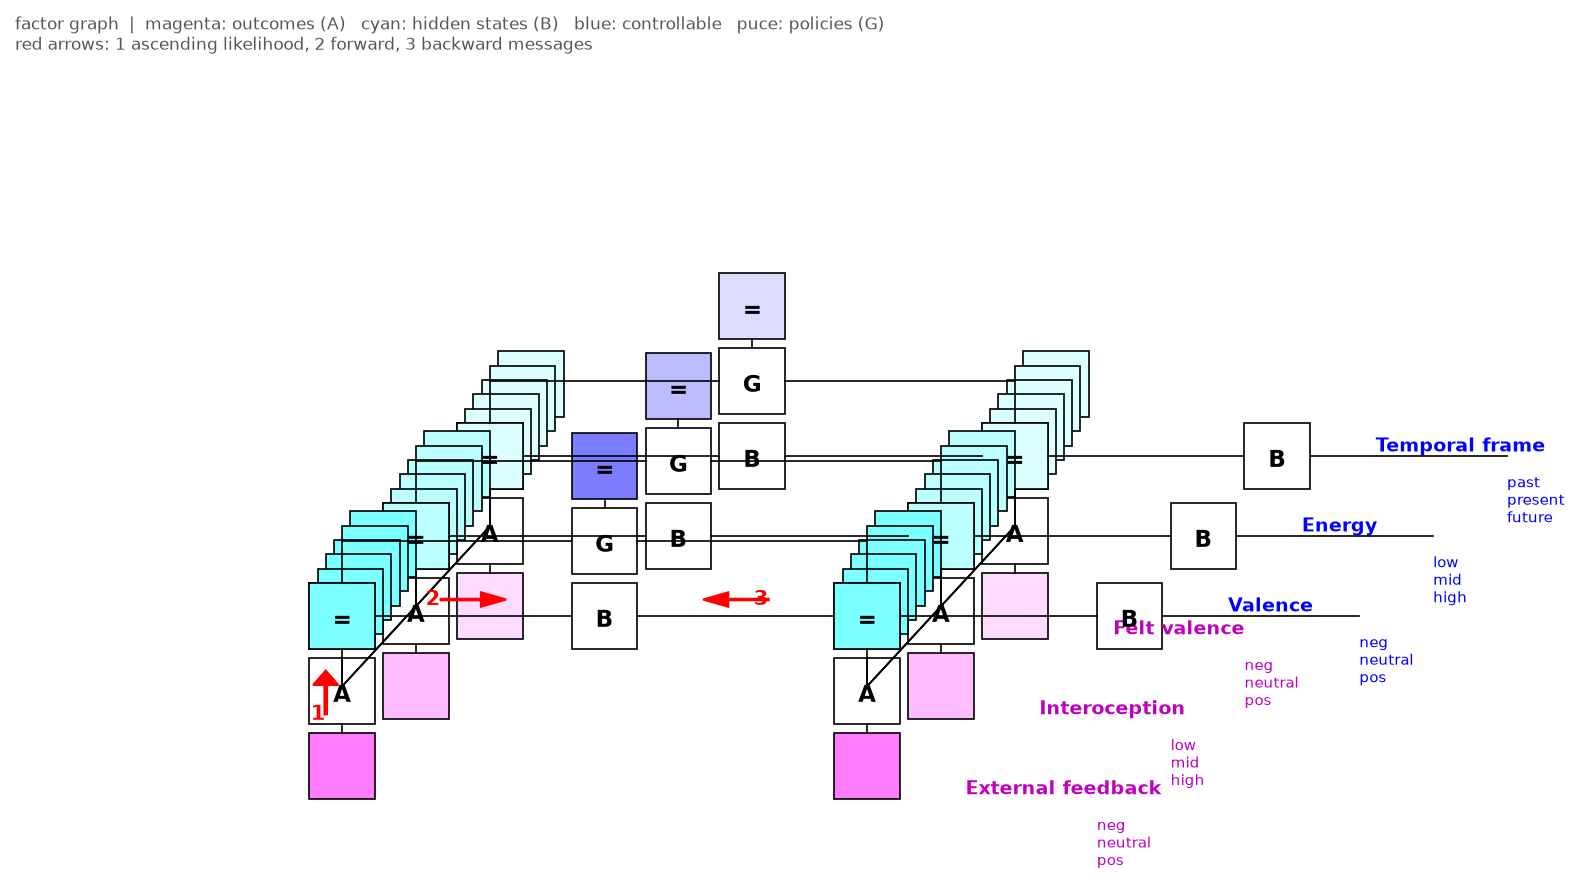
\includegraphics[width=\textwidth]{figures/fig_factor_graph.png}
\caption{\textbf{Factor graph of the generative model} (SPM convention: magenta =
outcome modalities with likelihood $\mathbf A$; cyan = hidden-state factors with
transition $\mathbf B$; controllable factors are stacks with policy and
expected-free-energy $G$ nodes; red arrows = message passing). Three controllable
factors (valence, energy, temporal frame) and three modalities integrate the
backward, present, and forward affective channels in one model.}
\label{fig:factorgraph}
\end{figure}

\subsection{Framing actions as temporal-precision operators}
Each action defines a transition $\mathbf B_a=\mathbf B_v^{(a)}\otimes\mathbf
B_e^{(a)}\otimes\mathbf B_f^{(a)}$, whose frame block $\mathbf B_f^{(a)}$ is a
\emph{temporal-precision operator} that redistributes probability across horizons. Six
actions realise the depth regulator:
\begin{description}
\item[RECALL] assigns $70\%$ self-transition to \textsc{past}; $\mathbf B_v^{\textsc{recall}}$
pulls valence toward a \emph{bidirectional} target $v_{\text{recall}}=0.2+0.6\alpha$
with $\alpha=\sigma(\pi_{\text{pos}}-\theta)$, so high positive-belief precision
$\pi_{\text{pos}}$ recalls a positive past (narrative stabilisation) and low
$\pi_{\text{pos}}$ a negative one (rumination). It is the computational realisation of
\emph{shallow}, identity-anchored retrieval (\S\ref{sec:regulator}).
\item[ENGAGE] assigns $75\%$ to \textsc{present}, maintaining precision on current
sensory input through perception--action coupling.
\item[FUTURATE] assigns $90\%$ to \textsc{future} (narrative inertia); $\mathbf
B_v^{\textsc{futurate}}$ pulls valence toward a \emph{precision-gated} target
$v_{\text{fut}}=0.2+0.6\alpha$, symmetric with RECALL, so high positive-belief
precision yields hopeful prospection and low precision yields anxious, worry-type
prospection rather than fixed optimism. Its energy cost brakes it into short reactive
planning bursts.
\item[FEEL] releases frame commitment ($50$--$60\%$ present) and models active
interoceptive processing, reducing accumulated prediction error through body-state
monitoring \citep{stephan2016allostatic}.
\item[DISSOCIATE] distributes probability roughly uniformly across frames, modelling
\emph{temporal unmooring} \citep{vannikov2018dissociation}.
\item[ABSTRACT] assigns $\approx60$--$80\%$ to \textsc{future}, an effortful,
ungrounded forward route that bypasses interoception and episodic recall.
\end{description}
$\mathbf B_{\text{frame}}$ matrices are additionally learned online via Dirichlet
updates, so agents acquire personalised temporal-attention operators. Here $\sigma$ is
the logistic function and $\theta=2$ the precision threshold; the exact frame- and
valence-transition entries, the channel temperatures $\tau_{\text{model}},
\tau_{\text{reward}}, \tau_{\text{action}}$, and the mood-layer constants are given in
the supplementary implementation (\texttt{generative\_model.py}, \texttt{agent.py}).

\subsection{Extensions and the mood layer}
Two extensions capture affective pathology. \emph{Asymmetric hedonic sensitivity}
replaces the scalar reward sensitivity with a pair $(c_{\text{pos}},c_{\text{neg}})$
scaling positive and negative preference entries separately, capturing dissociable
reward and punishment processing \citep{eshel2010reward,pizzagalli2014depression}.
\emph{Habit priors} add an additive log-prior $\mathbf E$ over policies
\citep{dacosta2020active}, so $\ln\pi(a)=-\gamma G(a)+E_a$, modelling EFE-suboptimal
habitual tendencies such as ruminative fixation \citep{watkins2008constructive}. A
hierarchical \emph{mood layer} (M5) infers $\pi_{\text{pos}}$ over slow timescales as
a categorical POMDP driven by accumulated believed-valence relative to neutral
\citep{eldar2016mood}, separating within-trial emotion from cross-trial mood
\citep{hesp2021deeply} and producing a self-reinforcing low-mood attractor under
vulnerability and stress from Bayesian inference alone (\S\ref{sec:dynamics}).

Table~\ref{tab:justification} maps each choice to its source; full detail is in
the supplementary design-justification document.

\begin{table}[htbp]
\centering\small
\caption{\textbf{Design justification (excerpt).} Predictive (P) and generative (G)
status flagged where the distinction applies.}
\label{tab:justification}
\begin{tabular}{p{3.3cm}p{6.0cm}p{3.7cm}}
\toprule
Choice & Rationale & Source \\
\midrule
Attention $=$ precision (P) & framing is precision redistribution over horizons & \citet{feldman2010attention} \\
Backward channel (P) & $-dF/dt$ valence & \citet{joffily2013emotional} \\
Present channel (P) & reward prediction error & \citet{pattisapu2024free} \\
Forward channel (P) & affective charge of policy revision (EFE) & \citet{hesp2021deeply} \\
Temporal-frame factor & mental time travel; shared memory/imagination machinery & \citet{schacter-addis2007,suddendorf-corballis1997} \\
Energy/interoception & allostatic body-budget & \citet{seth2016interoceptive,stephan2016allostatic} \\
RECALL (past) & self-memory system; overgeneral memory on failure & \citet{williams2007autobiographical} \\
Habit priors (E-vector) & habitual, EFE-suboptimal tendencies & \citet{dacosta2020active,watkins2008constructive} \\
Hedonic asymmetry (G) & reward/punishment sensitivity dissociate & \citet{eshel2010reward,pizzagalli2014depression} \\
Counterfactual emotions (G) & regret/relief from obtained vs foregone & \citet{hesp2020sophisticated} \\
Mood layer (M5) & mood/emotion timescale separation & \citet{hesp2021deeply,eldar2016mood} \\
Effort/energy cost & effortful deliberation carries a metabolic cost & \citet{treadway2009effort} \\
\bottomrule
\end{tabular}
\end{table}

\section{Three-channel valence and the temporal taxonomy}\label{sec:taxonomy}
The distribution of attention across horizons is a second-order inference, and the
three channels are read at successive stages of a single agent--environment cycle.
Updating beliefs from a new observation exposes the backward channel, model valence.
Comparing obtained against expected reward exposes the present channel, reward
valence. Revising the policy exposes the forward channel, action valence.

\subsection{The three channels}
\emph{Model valence} (backward) tracks $v_{\text{model}}=\tanh(-\Delta F/\tau_{\text{model}})$
\citep{joffily2013emotional}, modulating the model learning rate. \emph{Reward
valence} (present) is $v_{\text{reward}}=\tanh((U-\mathbb{E}[U])/\tau_{\text{reward}})$
over hedonic modalities \citep{pattisapu2024free}; interoceptive prediction errors
drive allostatic regulation but are excluded from felt valence. \emph{Action valence}
(forward) is $v_{\text{action}}=\tanh(\text{AC}/\tau_{\text{action}})$ with
$\text{AC}=(\boldsymbol\pi_{t-1}-\boldsymbol\pi_t)\cdot\mathbf G$
\citep{hesp2021deeply}, and feeds back on policy precision. This closes the
emotion--action loop: policy revision changes expected free energy, action changes
what is observed, and the resulting change in variational free energy feeds back
through $v_{\text{action}}$ onto the precision that governs the next policy.

\subsection{Composite valence and channel disagreement}
The channels combine as $V=\tanh(v_{\text{model}}+v_{\text{reward}}+v_{\text{action}})$.
Agreement yields unambiguous satisfaction or distress; disagreement is
informative. \emph{Productive failure} ($v_{\text{model}}<0$,
$v_{\text{action}}>0$): the outcome was bad but a better plan was found. \emph{Unsettling
success} ($v_{\text{reward}}>0$, $v_{\text{action}}<0$): good fortune that may not
last. \emph{Dawning anxiety} ($v_{\text{model}}\!\approx\!0$, $v_{\text{reward}}\!\approx\!0$,
$v_{\text{action}}<0$): nothing has happened, but plans are deteriorating.

\subsection{A worked example}
Take one trial of the gamble task-model of \S\ref{sec:empirical}. The agent gambles
and wins, and the win is larger than it expected. Read the channels in turn. The
present channel compares obtained reward with its expectation; the surplus makes
$v_{\text{reward}}>0$. The backward channel registers that the win improved model fit,
so $F$ fell and $v_{\text{model}}>0$. The forward channel registers that policy
precision has shifted toward gambling and that this lowered expected free energy, so
its affective charge $v_{\text{action}}>0$. All three agree, the composite
$V=\tanh(v_{\text{model}}+v_{\text{reward}}+v_{\text{action}})$ is strongly positive,
and the state is unambiguous satisfaction. Now change one thing: let the gamble lose,
but let the loss reveal that the safe option was the better policy. The present and
backward channels turn negative (the outcome was bad and fit worsened) while the
forward channel stays positive (a better plan was found). The channels disagree, and
the composite reports the muted, forward-leaning affect labelled productive failure
above. These three readings, taken at three stages of one inference cycle, are all the
taxonomy requires.

\subsection{The VFE/EFE temporal taxonomy of emotion}
Emotions inherit their temporal direction from whichever quantity generates them,
yielding a taxonomy we offer as an organising scheme rather than an essentialist
classification; its partitioning within an agent depends on developmental and
sociocultural history \citep{barrett2017theory}.
\emph{Backward} ($-dF/dt$, the rate of change of VFE): regret, guilt, shame, pride, gratitude.
\emph{Present} (RPE): joy, anger, disgust, surprise.
\emph{Forward} (EFE): hope, fear, anxiety, anticipation.
\emph{Transitional} (VFE vs prior EFE): relief, disappointment, satisfaction.
This grounds the temporal axis of appraisal theory
\citep{smith1985patterns,ortony1988cognitive} in a formal distinction rather than
folk labels.

\section{Prior models are special cases}\label{sec:predecessors}
Figure~\ref{fig:architecture} shows the architecture as a stack of layers and where
the prior models sit inside it. A task-specific generative model sits at the base:
states, observations, policies, and expected free energy for whatever task the agent
faces (the gamble task-model of \S\ref{sec:empirical}, an experience-sampling affect
model, any decision problem). On top of it sits the affective readout layer, the three
channels, whose composite feeds a represented valence state and a slow mood layer,
with the temporal-frame factor modulating precision across horizons. Each prior model
is one layer of this stack, and our contribution is the integration, not any single
channel.

The three predecessor accounts are \emph{reduced sub-graphs} of our model
(Figure~\ref{fig:submodels}, schematic): \citet{joffily2013emotional} is a
perception-only VFE model (one factor, no policy, backward channel only);
\citet{pattisapu2024free} is a single-factor POMDP with policy selection (present
channel, no temporal frame, no backward derivative); \citet{hesp2021deeply} is a deep
hierarchical model carrying the forward affective-charge channel and a slow mood layer,
but without a reward decomposition or a temporal-frame factor. Each predecessor
contributes at most one of our affective channels, and we make the debt explicit: the
mood layer that carries our diathesis-stress dynamics is adopted from
\citet{hesp2021deeply} (with its evidence changed from free energy to valence,
\S\ref{sec:dynamics}). The contribution is thus an integration, a task-specific
model, and an inferred temporal frame that none of the three has, not a claim to
have out-built any one of them on its own terrain; \S\ref{sec:empirical} shows the
channel decomposition precisely.

\begin{figure}[htbp]
\centering
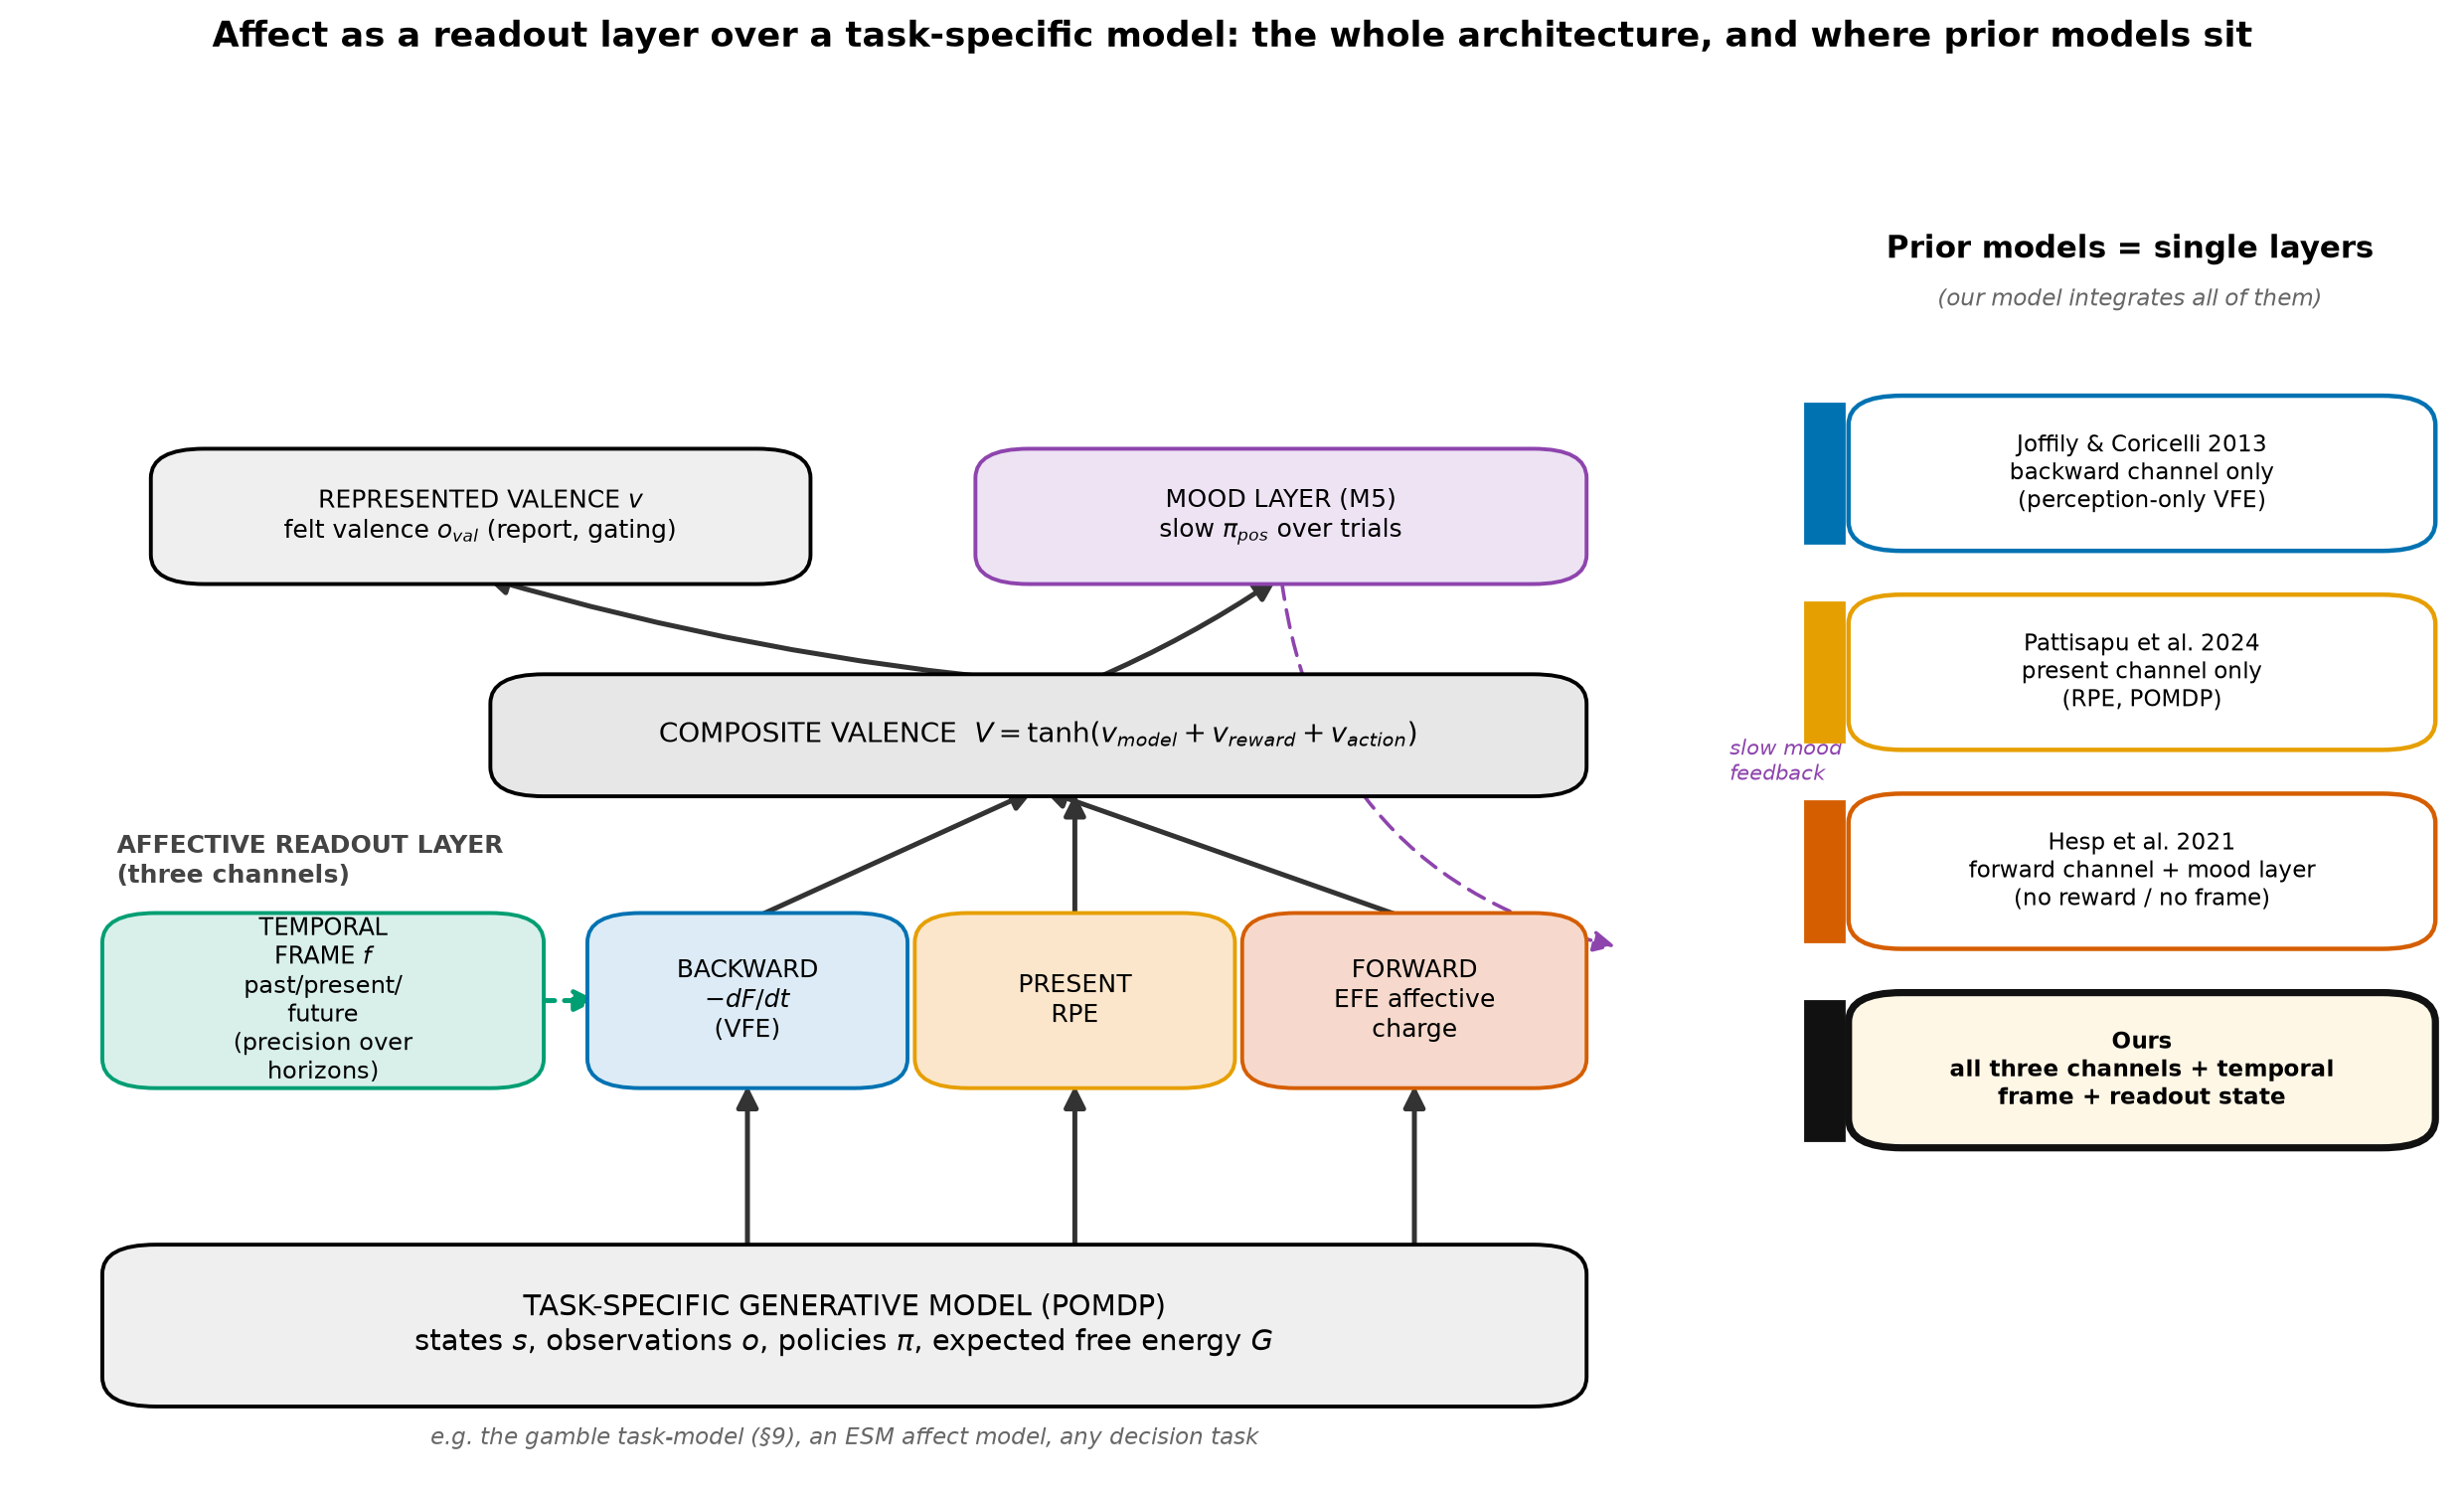
\includegraphics[width=\textwidth]{figures/fig_architecture.png}
\caption{\textbf{The layered architecture, and where prior models sit.} Affect is a
readout layer over a task-specific generative model (base). The three channels
(backward, present, forward) read off the dynamics of inference; their composite feeds
a represented valence state and a slow mood layer, with the temporal-frame factor
modulating precision across horizons. Each prior model corresponds to a single layer:
Joffily \& Coricelli to the backward channel, Pattisapu et al.\ to the present
channel, Hesp et al.\ to the forward channel plus mood layer. Our model integrates all
of them and adds the temporal-frame factor and the readout state.}
\label{fig:architecture}
\end{figure}

\begin{figure}[htbp]
\centering
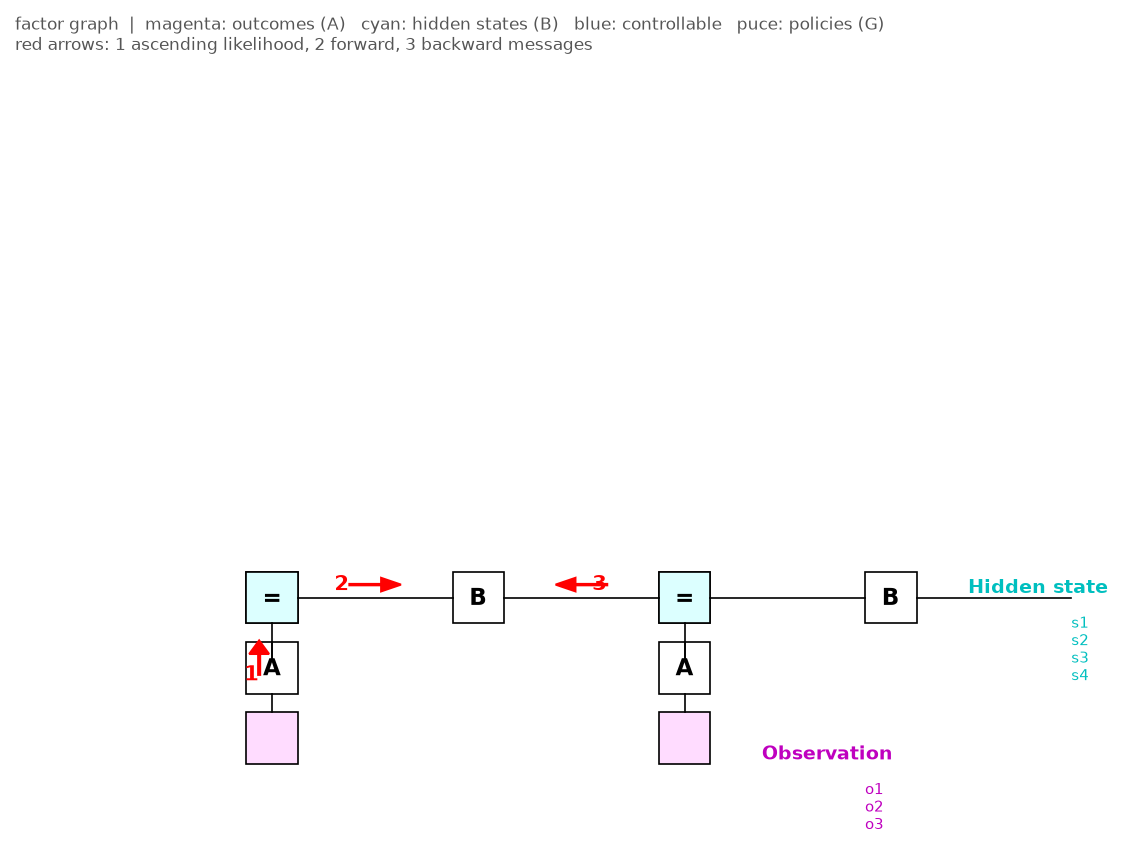
\includegraphics[width=0.32\textwidth]{figures/fig_submodel_joffily.png}\hfill
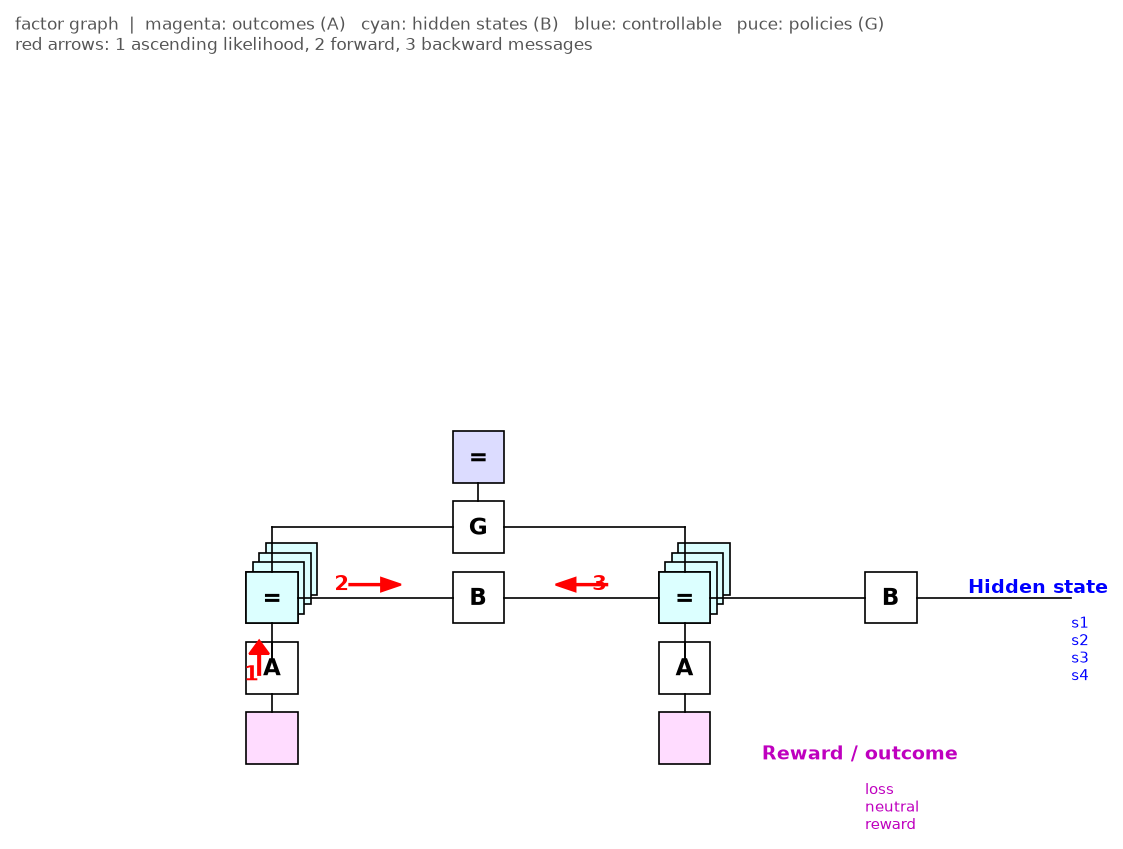
\includegraphics[width=0.32\textwidth]{figures/fig_submodel_pattisapu.png}\hfill
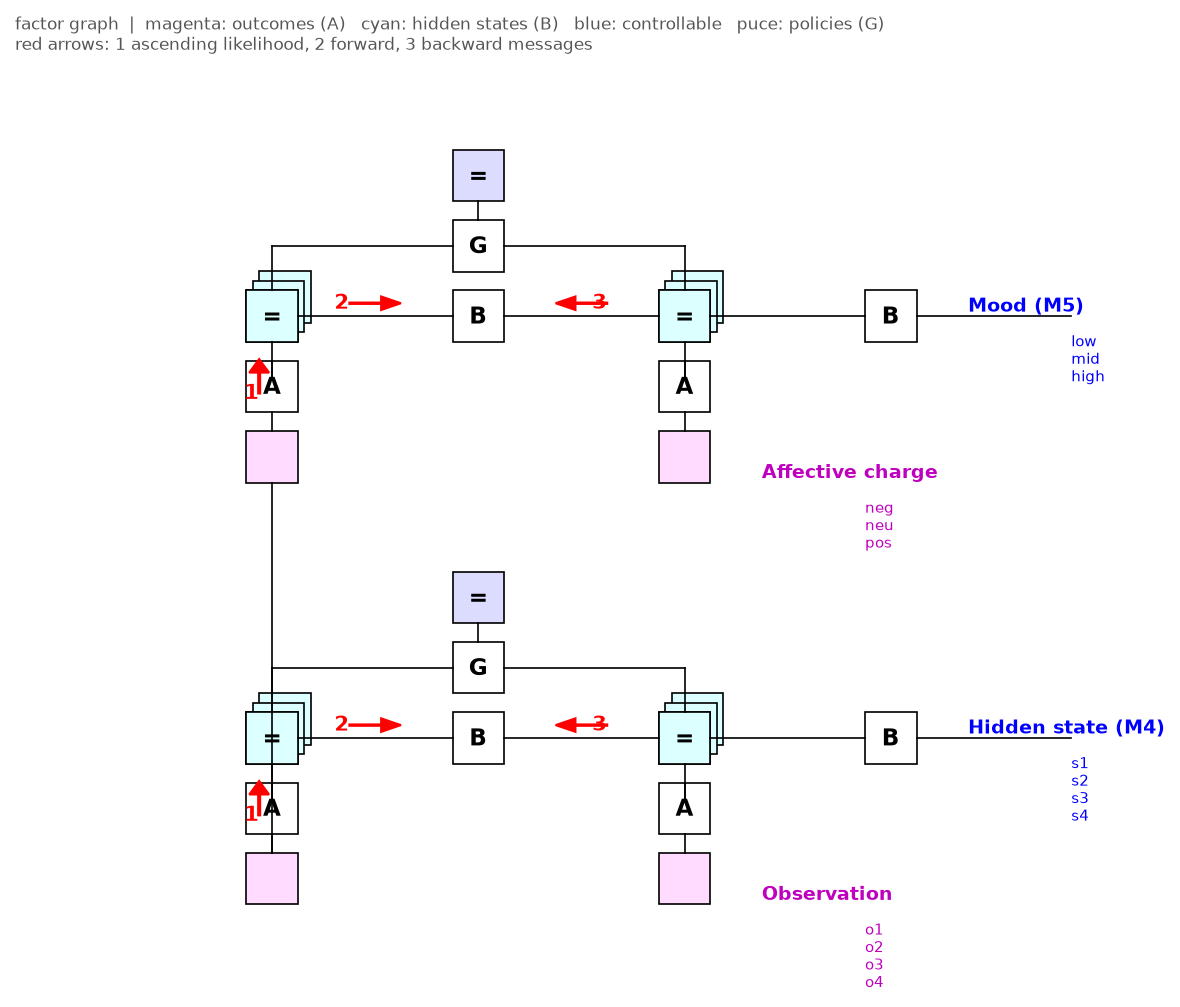
\includegraphics[width=0.32\textwidth]{figures/fig_submodel_hesp.png}
\caption{\textbf{Predecessor models as reduced factor graphs.} Joffily \& Coricelli
(backward, perception-only); Pattisapu et al. (present, single-factor POMDP); Hesp
et al. (forward, deep hierarchy). Each captures one channel; none has the
temporal-frame factor of Figure~\ref{fig:factorgraph}.}
\label{fig:submodels}
\end{figure}

\section{Temporal framing dynamics: self-regulation vs self-amplification}\label{sec:dynamics}
Adaptive flexibility is the capacity to move between framing modes as the situation
demands. The loop admits two regimes. Under \emph{self-regulation} it is
homeostatic. High VFE triggers corrective action, and positive $v_{\text{action}}$
sharpens precision on the corrective trajectory. Under \emph{self-amplification} it is
pathological. Framing locks into a single mode; precision on that mode's errors
intensifies, and the agent cannot update away. We illustrate the dynamics across three
parameter phenotypes used in Figure~\ref{fig:framing}: a \emph{healthy} agent (high
$\pi_{\text{pos}}$, intact interoception), a \emph{depressive} one (low $\pi_{\text{pos}}$,
blunted reward sensitivity), and a \emph{manic} one (low interoceptive precision and
disinhibited forward framing).

\subsection{RECALL supports engagement, and its feedback reliance}
Past-oriented framing is preparatory: RECALL stabilises beliefs by pulling toward the
prior, lowering VFE and making ENGAGE more competitive, so a RECALL-to-ENGAGE
pipeline emerges in healthy agents (Figure~\ref{fig:framing}d,e). This capacity is
constrained by feedback. When $\pi_{\text{pos}}$ is low, RECALL fails at two coupled
levels: the mechanism itself is impaired ($\alpha\!\approx\!0.14$, barely pulling
toward the prior) and its deployment is suppressed (it becomes EFE-uncompetitive).
Figure~\ref{fig:feedback} contrasts a healthy and a recall-impaired agent differing
only in $\pi_{\text{pos}}$: RECALL utilisation collapses from $26\%$ to $<1\%$, with
compensatory FEEL, ENGAGE, and ABSTRACT. This is the computational form of
overgeneral memory \citep{williams2007autobiographical}: cognition migrates to
representations that are abstract without being self-congruent.

\begin{figure}[htbp]
\centering
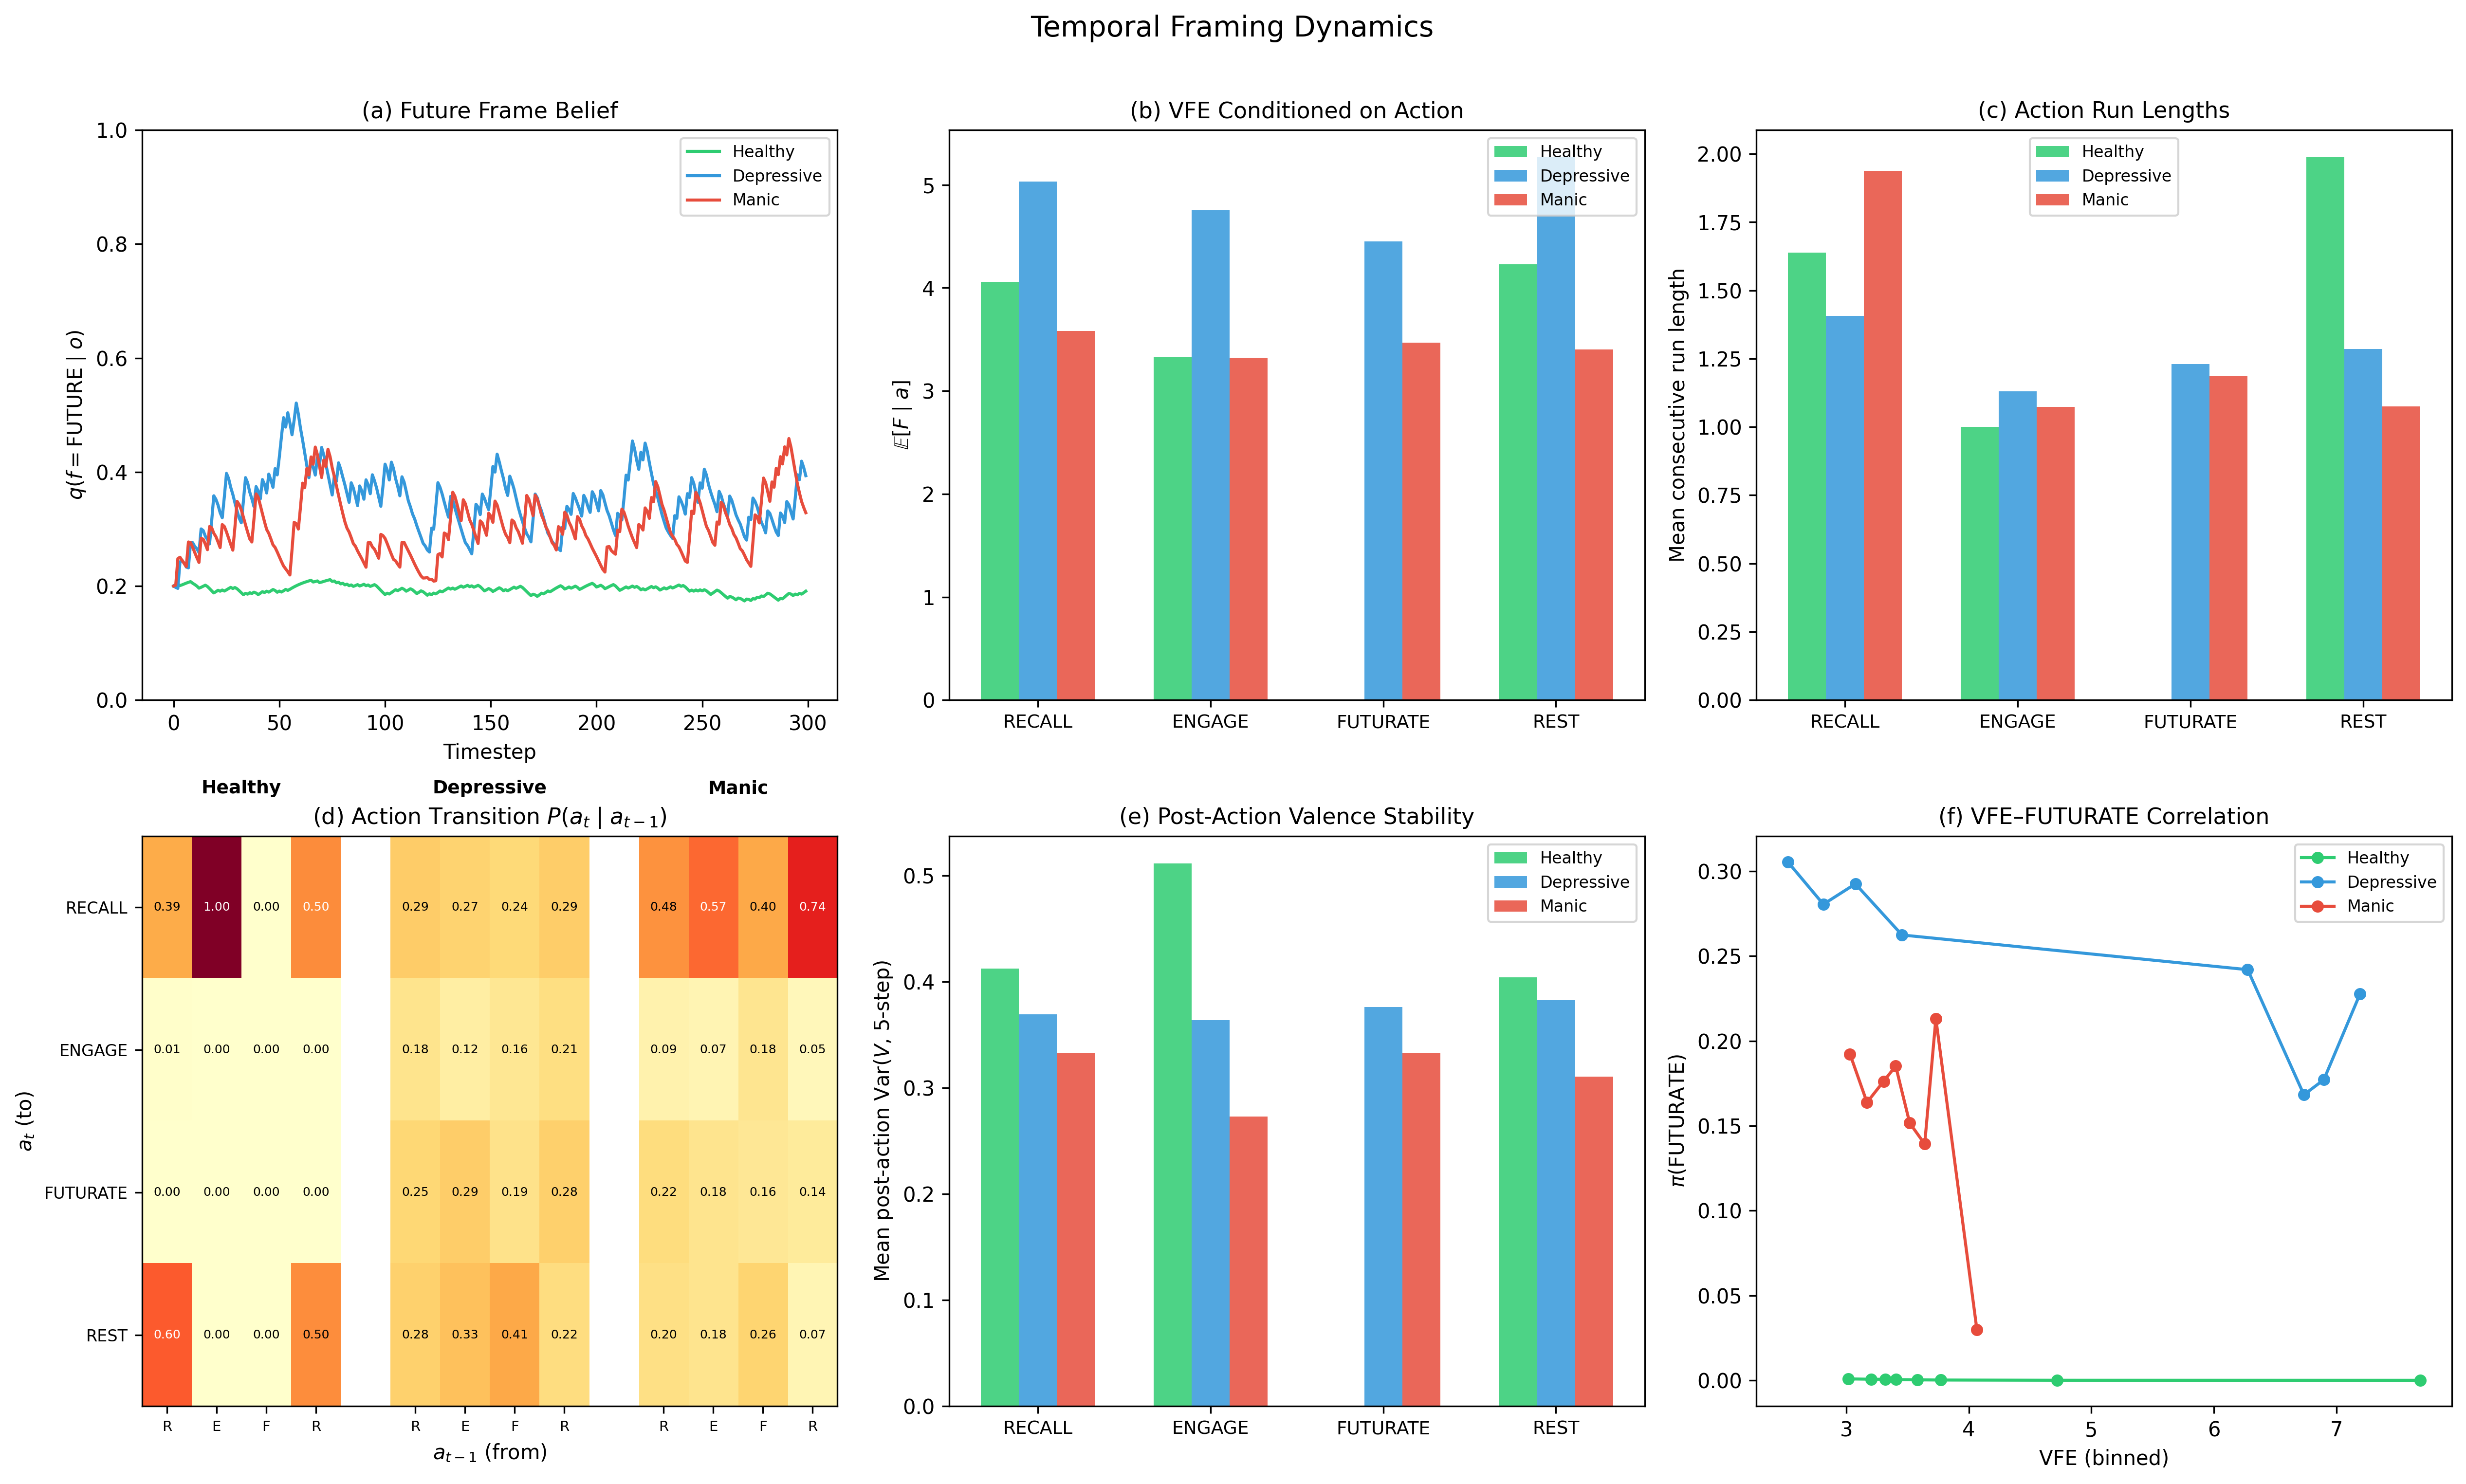
\includegraphics[width=\textwidth]{figures/fig11_framing_dynamics.png}
\caption{\textbf{Temporal framing dynamics.} (a) Future-frame belief over time per
profile. (b) Mean VFE conditioned on the selected action. (c) Action run lengths
(ABSTRACT and DISSOCIATE longest in the manic profile). (d) Action transition matrices:
the RECALL-to-ENGAGE pipeline in healthy agents. (e) Post-action valence stability:
RECALL lowest. (f) Forward-framing tendency ($\pi(\textsc{futurate})+\pi(\textsc{abstract})$,
the two future-pulling operators, of which ABSTRACT carries most of the mass) against
within-profile VFE percentile. FUTURATE itself is a rare, high-cost reactive-planning
burst; ABSTRACT is the low-cost operator that does most forward framing.}
\label{fig:framing}
\end{figure}

\begin{figure}[htbp]
\centering
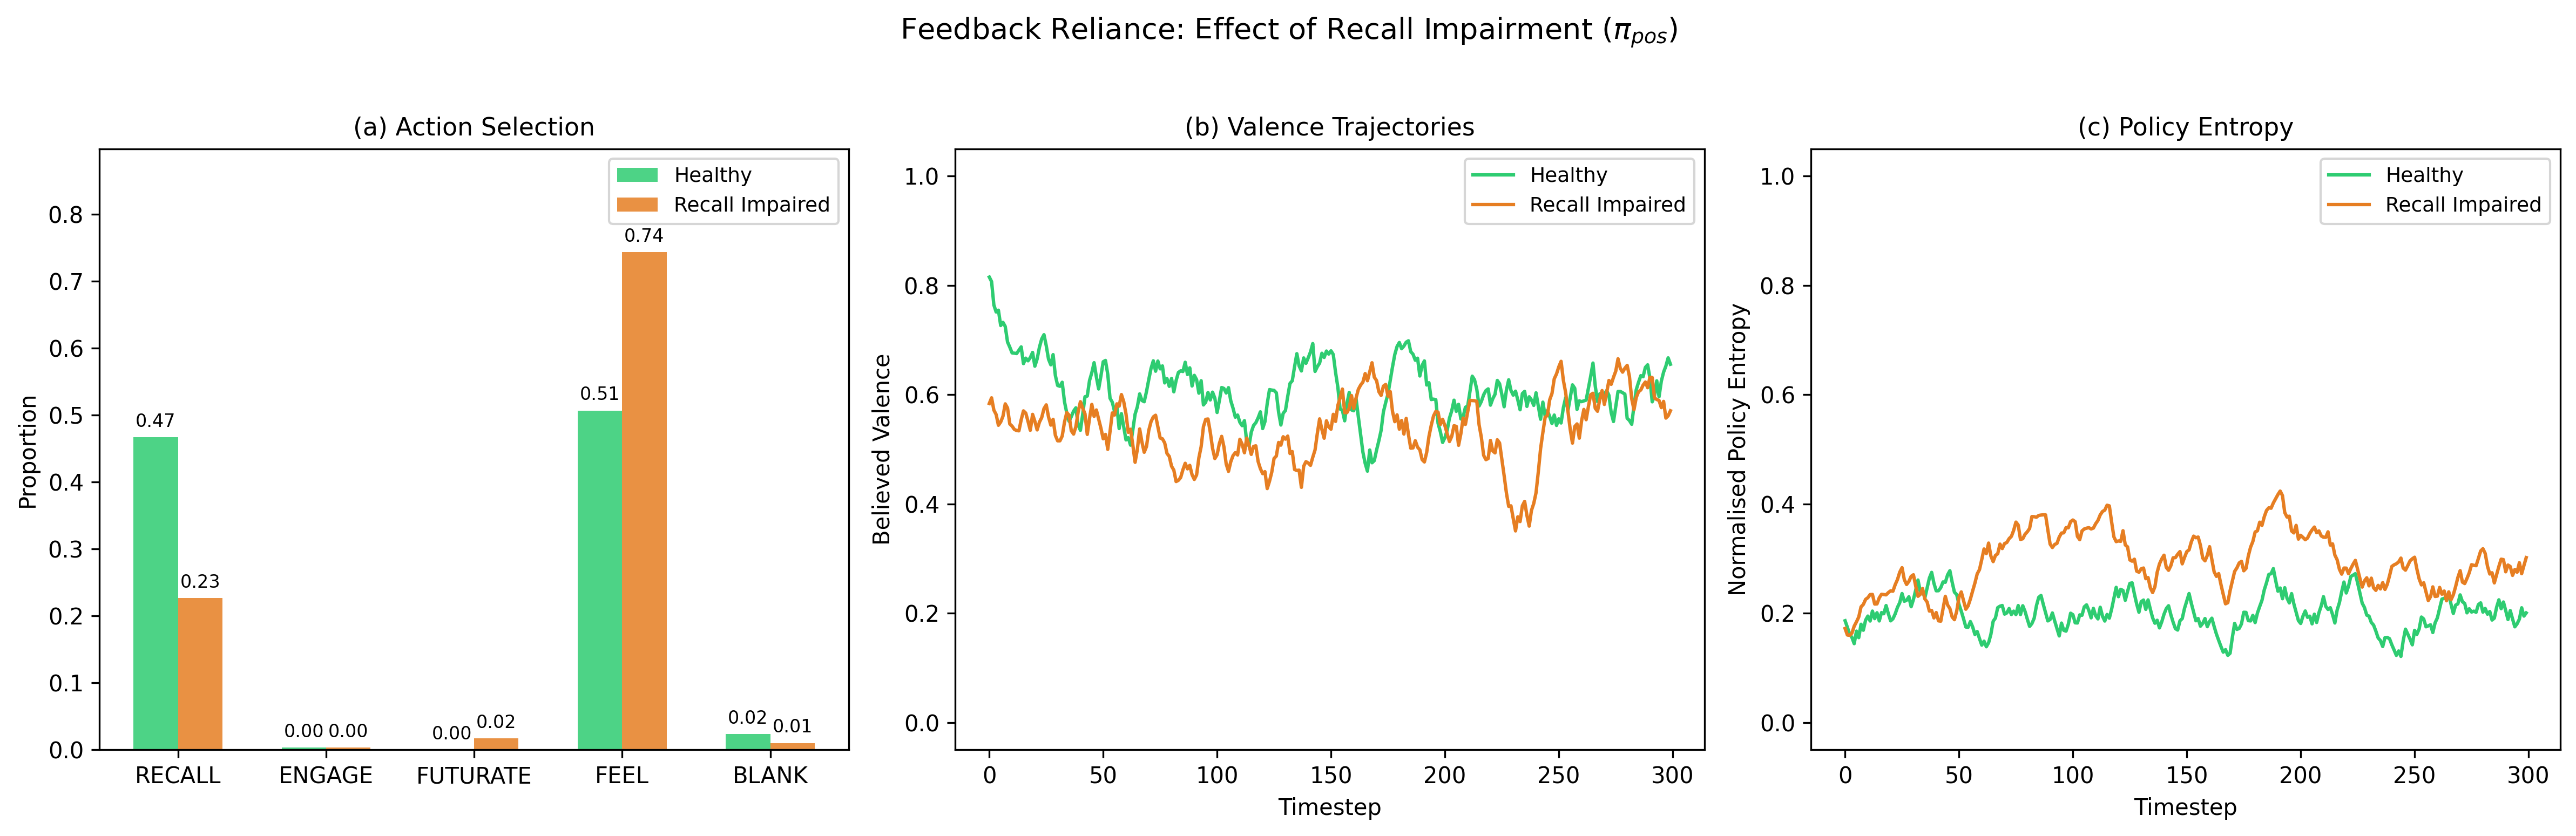
\includegraphics[width=\textwidth]{figures/fig10_feedback_reliance.png}
\caption{\textbf{Feedback reliance under recall impairment.} Profiles share all
parameters except $\pi_{\text{pos}}$ (5.0 vs 0.2). (a) RECALL drops from $26\%$ to
$<1\%$, with compensatory FEEL/ENGAGE/ABSTRACT. (b) Valence trajectories
lower under impairment. (c) Policy entropy: the impaired agent is less decisive.}
\label{fig:feedback}
\end{figure}

\subsection{Chronic stress as maladaptive temporal fixation}
Chronic stress realises the double bind of \S\ref{sec:regulator}. Affect turns
negative but construal stays coarse, so neither pathway to policy selection delivers.
A stressed profile (very high volatility, amplified reward sensitivity, stress-impaired
interoception, reduced $\pi_{\text{pos}}$) shows future-dominated fixation, dominant
\textsc{future} frame belief ($0.57$ vs $0.32$ healthy), depleted \textsc{present}
($0.32$ vs $0.46$), forward-framing dominance (ABSTRACT, the low-cost prospection
operator, taken on $66\%$ of steps), and negative reward valence
($-0.35$ vs $+0.06$ healthy) from \emph{frustrated forward projection}: abstract
prospection commits to above-neutral predictions that a volatile world falsifies
(Figure~\ref{fig:stress}). The direction of these effects holds across seeds.

At the slow mood timescale, the M5 layer accumulates believed-valence evidence, so
persistently below-neutral affect drives positive-belief precision $\pi_{\text{pos}}$
below the rumination knee, where RECALL turns to rumination and sustains the low-mood
state. This produces a \emph{diathesis-stress} pattern rather than a stress-alone one
(Figure~\ref{fig:mood}). Crossing vulnerability (low $\pi_{\text{pos}}$, blunted reward
sensitivity, weak interoception) against chronic stress (high volatility) in a $2\times2$
design, only the conjunction collapses. Across eight seeds a healthy agent stays high
even under chronic stress (final $\pi_{\text{pos}}=5.2\pm0.7$, depressed in $0/8$),
vulnerability alone recovers ($4.2\pm1.0$, $0/8$), and only the vulnerable agent under
stress falls into a self-sustaining depressive attractor ($0.8\pm0.2$, $8/8$ below the
knee). Neither factor alone suffices, matching the diathesis-stress account of
depression \citep{monroe1991diathesis} and the resilience of most people to stress. We
present this as a mechanistic demonstration, not evidence: the parameters instantiate
vulnerability rather than fit it. It makes a falsifiable prediction: in longitudinal
experience-sampling, the interaction of vulnerability and stress, not either main
effect, should predict transition into sustained low mood, and the transition should be
preceded by a persistent below-neutral shift in momentary valence rather than in
prediction error.

\begin{figure}[htbp]
\centering
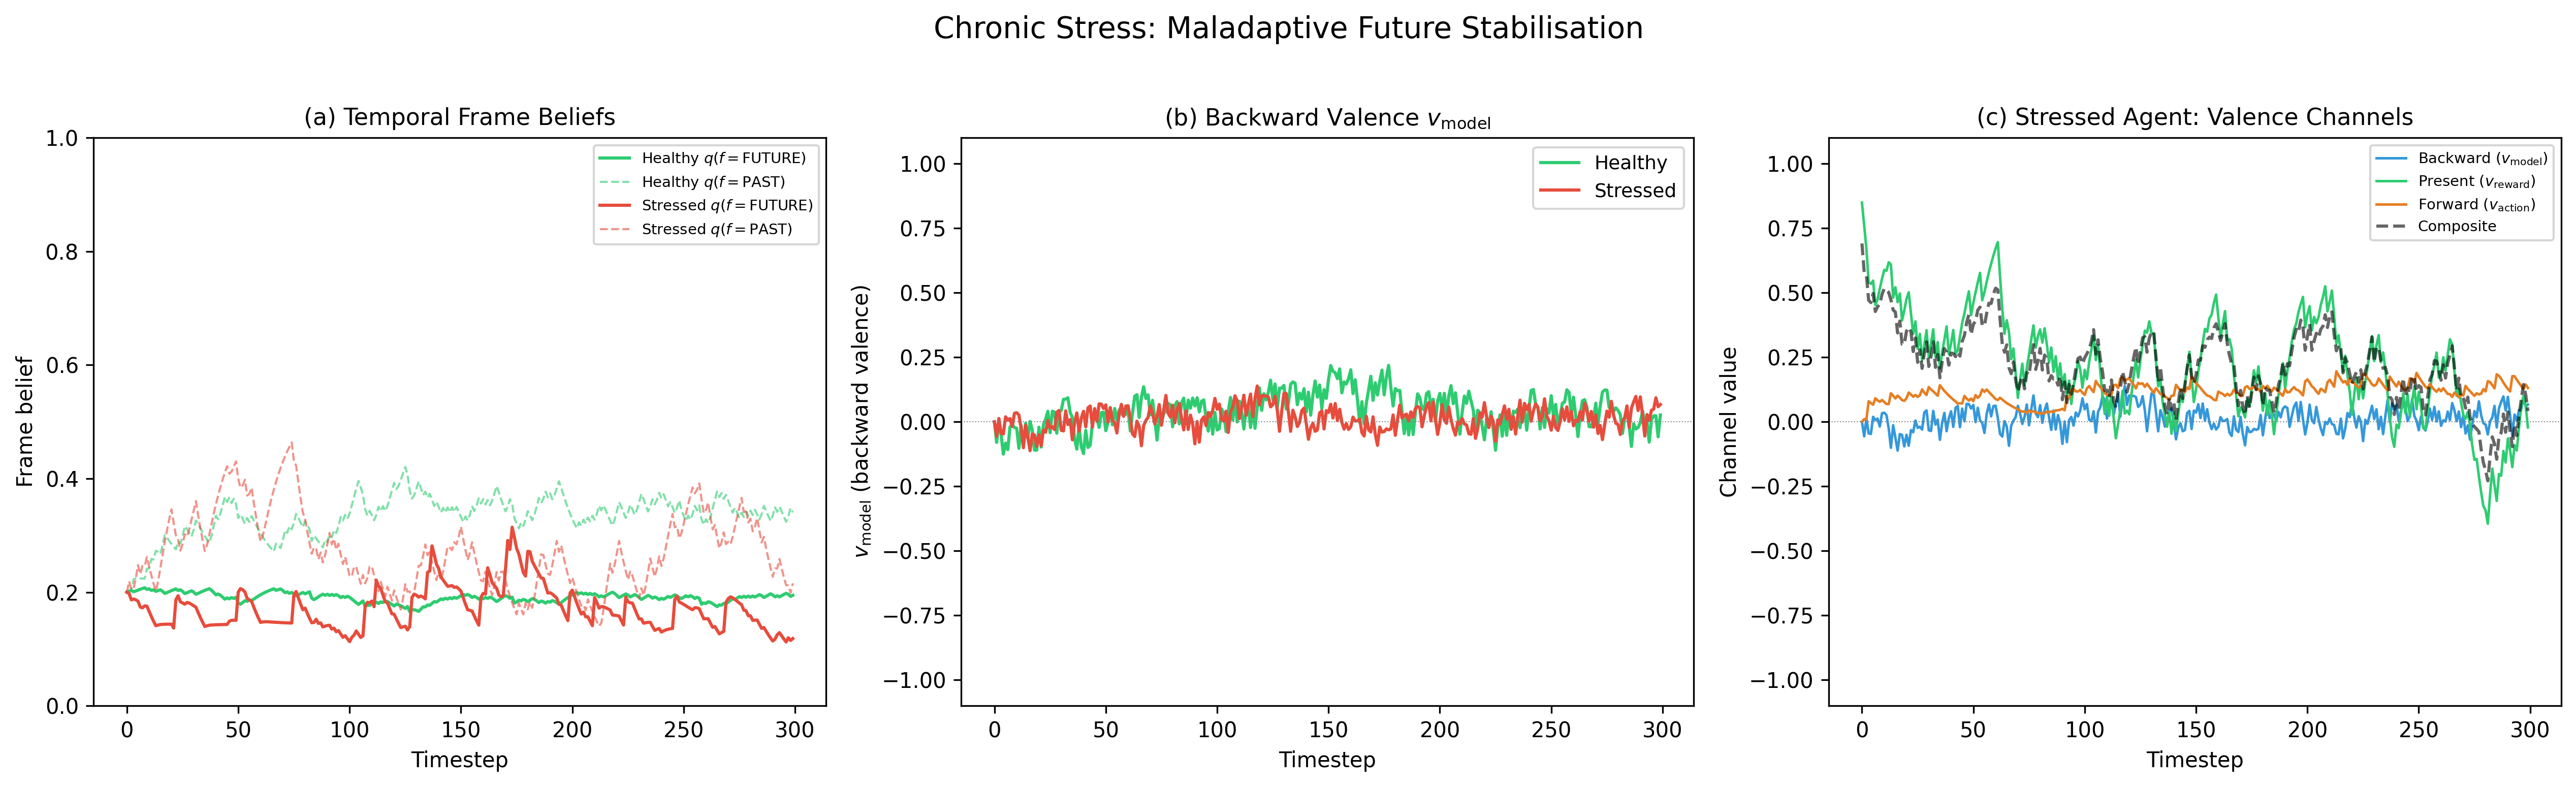
\includegraphics[width=\textwidth]{figures/fig12_chronic_stress.png}
\caption{\textbf{Chronic stress as maladaptive temporal fixation.} Stressed vs healthy.
(a) Frame beliefs: dominant \textsc{future}, depleted \textsc{present}. (b) Backward
valence more variable under high volatility. (c) Channel decomposition: negative
reward valence drives composite valence down via frustrated forward projection.}
\label{fig:stress}
\end{figure}

\begin{figure}[htbp]
\centering
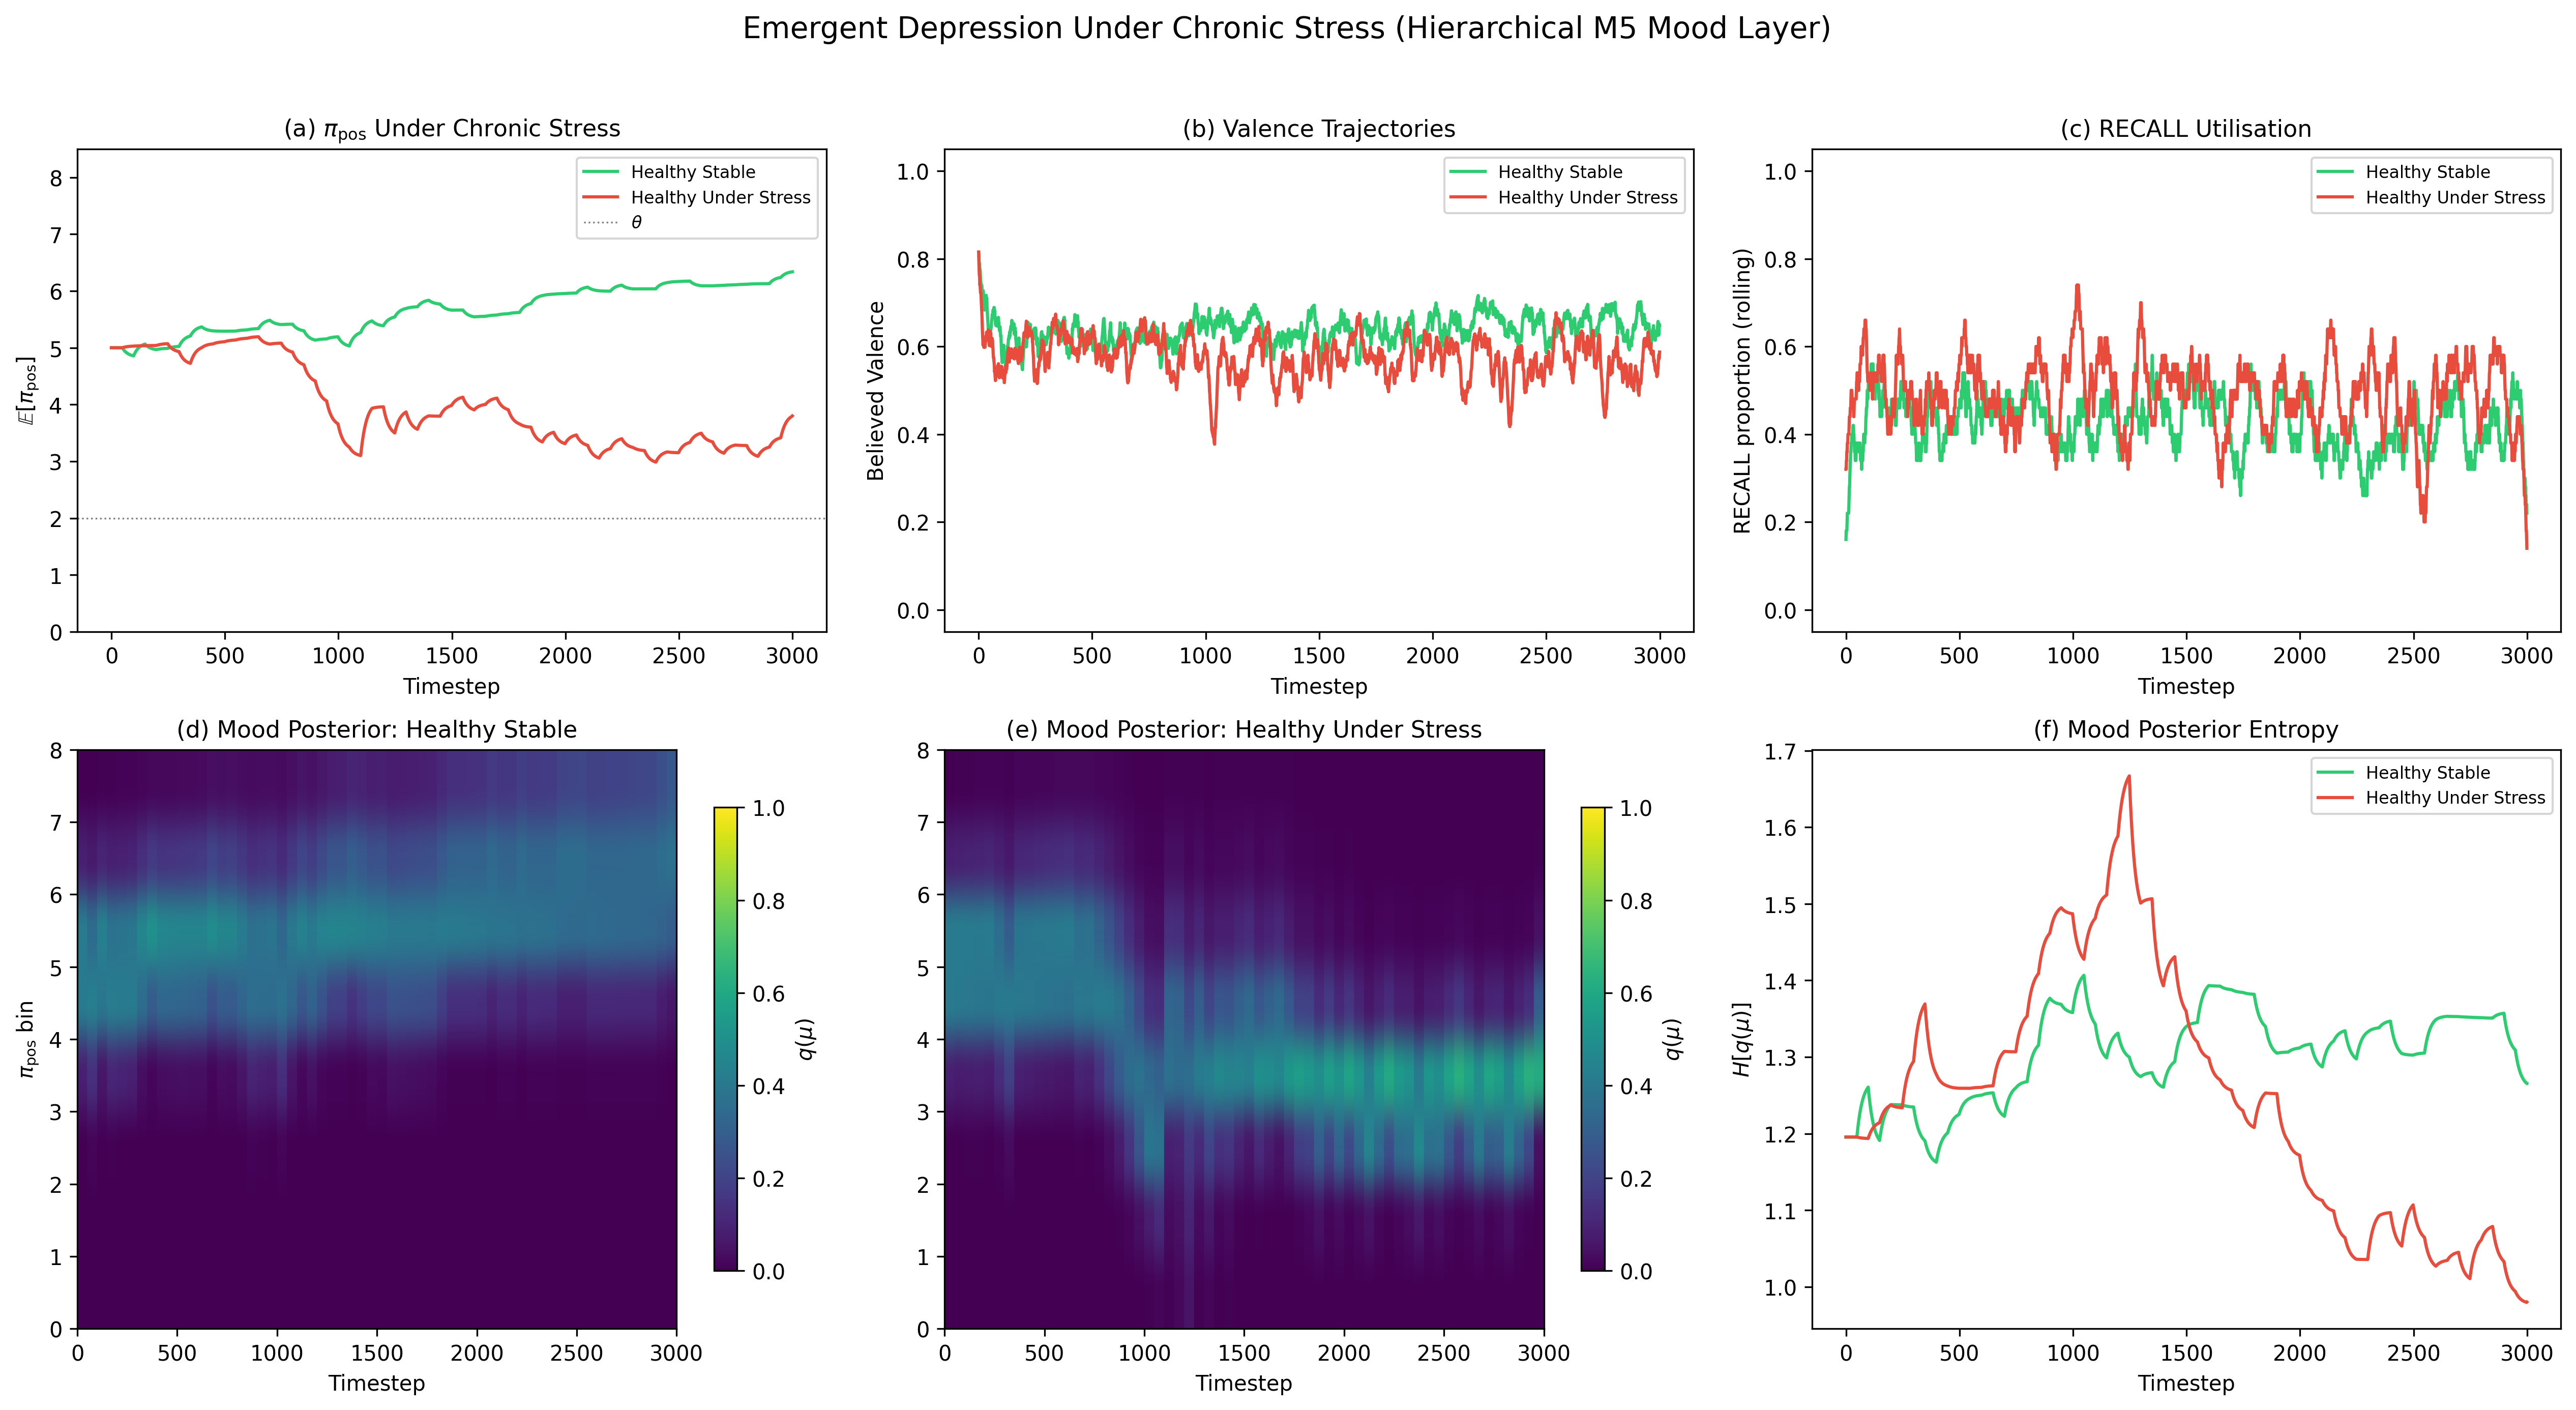
\includegraphics[width=\textwidth]{figures/fig14_stress_decay.png}
\caption{\textbf{Diathesis-stress in the M5 mood layer.} A $2\times2$ design crosses
vulnerability (low $\pi_{\text{pos}}$, blunted reward sensitivity, weak interoception)
with chronic stress (high volatility). (a) Mood ($\mathbb{E}[\pi_{\text{pos}}]$)
trajectories; (b) believed valence, the mood evidence, relative to neutral (dotted).
(c) Final mood by condition: only vulnerability $\times$ stress crosses the rumination
knee ($\theta=2$). (d) The vulnerable-under-stress mood posterior collapses to the low
bin; (e) the healthy-under-stress posterior stays high (resilience). (f) Mood-posterior
entropy. Robust across seeds (vulnerable$+$stress depressed $8/8$; others $0/8$).
$T=3000$.}
\label{fig:mood}
\end{figure}

\section{Counterfactual emotions (a generative mechanism)}\label{sec:counterfactual}
Regret and relief require comparing what happened with what \emph{would} have
happened. Adapting the counterfactual free-energy machinery of
\citet{hesp2020sophisticated}, we write
$\text{Regret}=F_{\text{actual}}-\min_{\pi'}F_{\text{counterfactual}}(\pi')$.
Computing $F_{\text{counterfactual}}$ requires running
the generative model offline, exactly what temporal framing does. This mechanism makes
a behavioural prediction that a reward-only model cannot. Across 143 participants, a
better \emph{foregone} outcome drives switching on the next choice over and above one's
own outcome ($t=10.4$; $P(\text{switch}\mid\text{regret})=0.45$ vs
$P(\text{switch}\mid\text{relief})=0.26$; Figure~\ref{fig:cf}), a dissociation a
factual (no-counterfactual) model has no way to produce. The same switching signature
replicates on a second complete-feedback dataset \citep{palminteri2017confirmation}
($n=20$). What the counterfactual term
does \emph{not} do is improve the prediction of affect magnitude or choice likelihood:
on complete-feedback choice data and on large-scale affect data it is redundant with
the reward-prediction signal (\S\ref{sec:empirical}). We therefore class it as a
grounded generative mechanism with a specific behavioural signature, not a general
predictive-fit improver.

\begin{figure}[htbp]
\centering
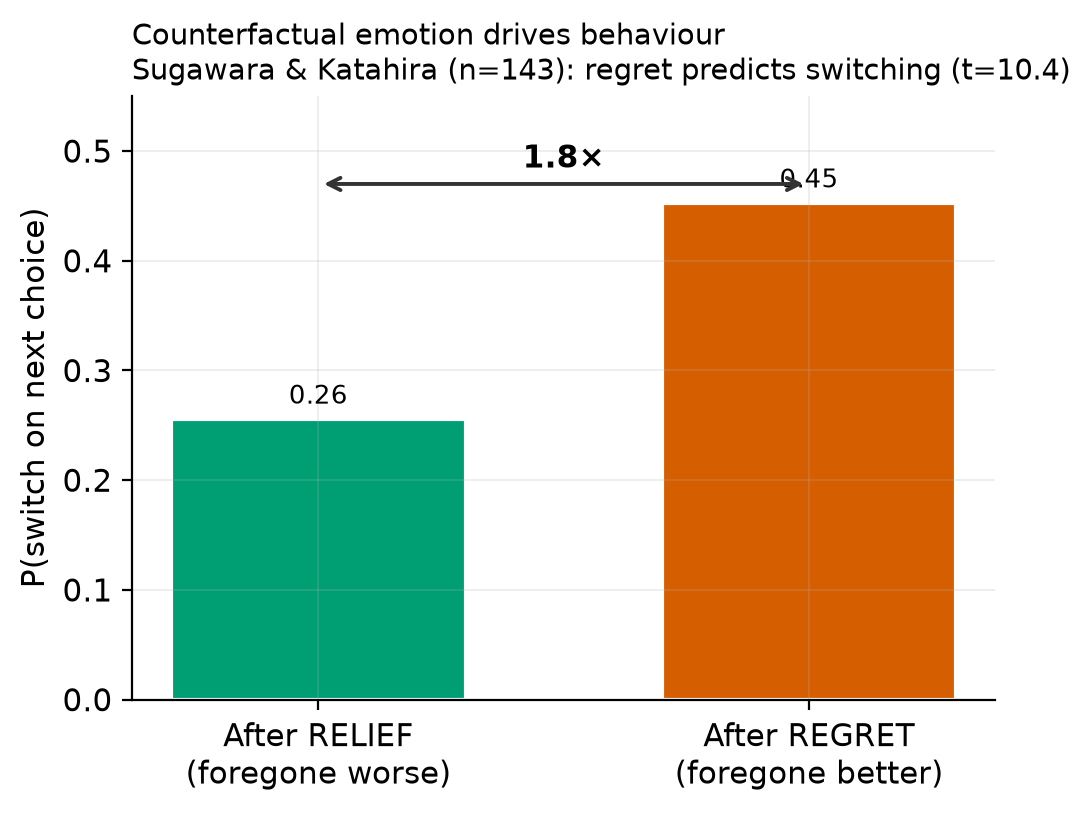
\includegraphics[width=0.5\textwidth]{figures/fig_counterfactual_signature.png}
\caption{\textbf{Counterfactual emotion drives behaviour.} People switch $\sim$1.7$\times$
more after regret than relief (\citealp{sugawara2021dissociation}, $n=143$), a signature a
factual model cannot generate. This validates the mechanism as the generator of
regret/relief, independent of its (null) contribution to prediction.}
\label{fig:cf}
\end{figure}

\section{Empirical validation: head-to-head and extension}\label{sec:empirical}
We tested the model on open data, holding out participants throughout. Provenance,
scripts, and full results are in the supplementary \texttt{EMPIRICAL\_RECORD.md};
Table~\ref{tab:datasets} lists the datasets and what each supports.

\begin{table}[htbp]
\centering\small
\caption{\textbf{Datasets.} $N$ is participants (held-out analysis subset in
parentheses); ES = effect sizes.}
\label{tab:datasets}
\begin{tabular}{p{3.4cm}p{2.0cm}p{4.4cm}p{1.7cm}p{2.6cm}}
\toprule
Dataset & $N$ & Signals & Access & Supports \\
\midrule
Rutledge GBE happiness \citep{rutledge2014} & 47{,}067 (14{,}803) & gamble choices; momentary happiness & CC0 (Dryad) & subsumption / affect readout \\
Geschwind--Bringmann ESM \citep{bringmann2013,geschwind2011} & 130 (129) & momentary affect; event pleasantness; worry & CC BY-NC & affect-dynamics; frame-to-worry \\
Reliability ESM (\texttt{osf.io/83cfk}) & 91 & momentary affect (12 emotion sliders) & open (OSF) & affect-dynamics replication \\
Temporal-orientation ESM \citep{mulholland2023} & 101 & per-probe past/future thought; valence & CC BY-NC & direct frame-to-affect coupling \\
Sugawara \& Katahira \citep{sugawara2021dissociation} & 143 & choices; obtained + foregone outcomes & open (OSF) & counterfactual signature \\
Palminteri et al.\ \citep{palminteri2017confirmation} & 20 & choices; obtained + foregone outcomes & open (OSF) & counterfactual replication \\
Reward+punishment reversal (osf.io/2gq96) & 128 (64/64) & learning rates by valence & open (OSF) & general precision deficit \\
Reward Positivity (MEG) \citep{pirrung2025} & 90 (52/38) & neural reward response & CC0 & reward reactivity ($c_{\text{pos}}$) \\
\bottomrule
\end{tabular}
\end{table}

\subsection{Subsumption: our affect layer recovers the happiness equation}
We instantiate our
three channels over a \emph{gamble} task-model (policies $\{$safe, gamble$\}$;
preferences increasing in reward) for the Great Brain Experiment happiness data
\citep{rutledge2014} ($47{,}067$ participants; evaluated held out across a
$14{,}803$-participant subset, $96{,}624$ held-out ratings). We reconstruct each
predecessor as its single affective channel over this shared task-model (single-channel
reconstructions, not the authors' original implementations) and compare them against the
integrated readout on the same held-out ratings (the task-model is
Figure~\ref{fig:gamble}, its combination with the emotion model is
Figure~\ref{fig:gamblecombined}; results in Table~\ref{tab:headtohead} and
Figure~\ref{fig:advantage}A). No single channel reproduces the integrated result. The
present channel (Pattisapu, RPE) reaches $R^2=0.111$ and the forward channel (Hesp, EFE)
$R^2=0.034$, while the backward channel (Joffily, $-dF/dt$) scores $R^2=0.000$. The last
is expected rather than a defeat: a rate-of-change signal cannot predict a happiness
\emph{level} on a single-shot gamble that has no temporal dynamics to track. The
integrated model reaches $R^2=0.144$, recovering the standard happiness equation
(CR$+$EV$+$RPE, $R^2=0.146$). No expected-value term is entered as a regressor; expected
value instead emerges from the forward/EFE channel, which on this task encodes
anticipated reward by construction, and adding it to the present channel raises $R^2$
from $0.111$ to $0.144$ ($+30\%$). The happiness equation is thus a special case of our
framework.

\begin{figure}[htbp]
\centering
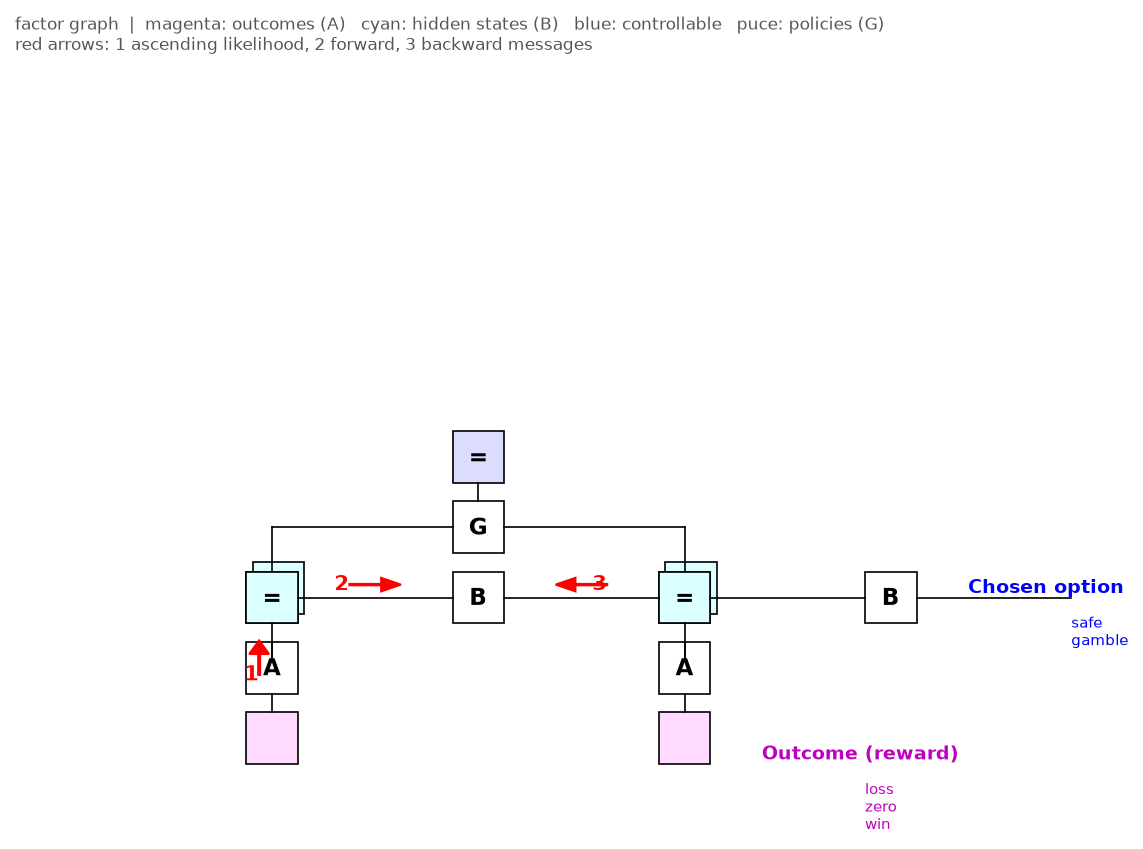
\includegraphics[width=0.68\textwidth]{figures/fig_gamble_taskmodel.png}
\caption{\textbf{The gamble task-model used for the subsumption test.} The
task-specific generative model over which the affect channels are read out: a single
reward-outcome modality (loss/zero/win) generated by the chosen option (safe/gamble),
with a preference gradient increasing in reward. Affect is a readout layer over this
model, and each predecessor corresponds to one channel of that readout. This is the
gambling-task instance of the general architecture in Figure~\ref{fig:factorgraph};
Figure~\ref{fig:gamblecombined} shows the two joined.}
\label{fig:gamble}
\end{figure}

\begin{figure}[htbp]
\centering
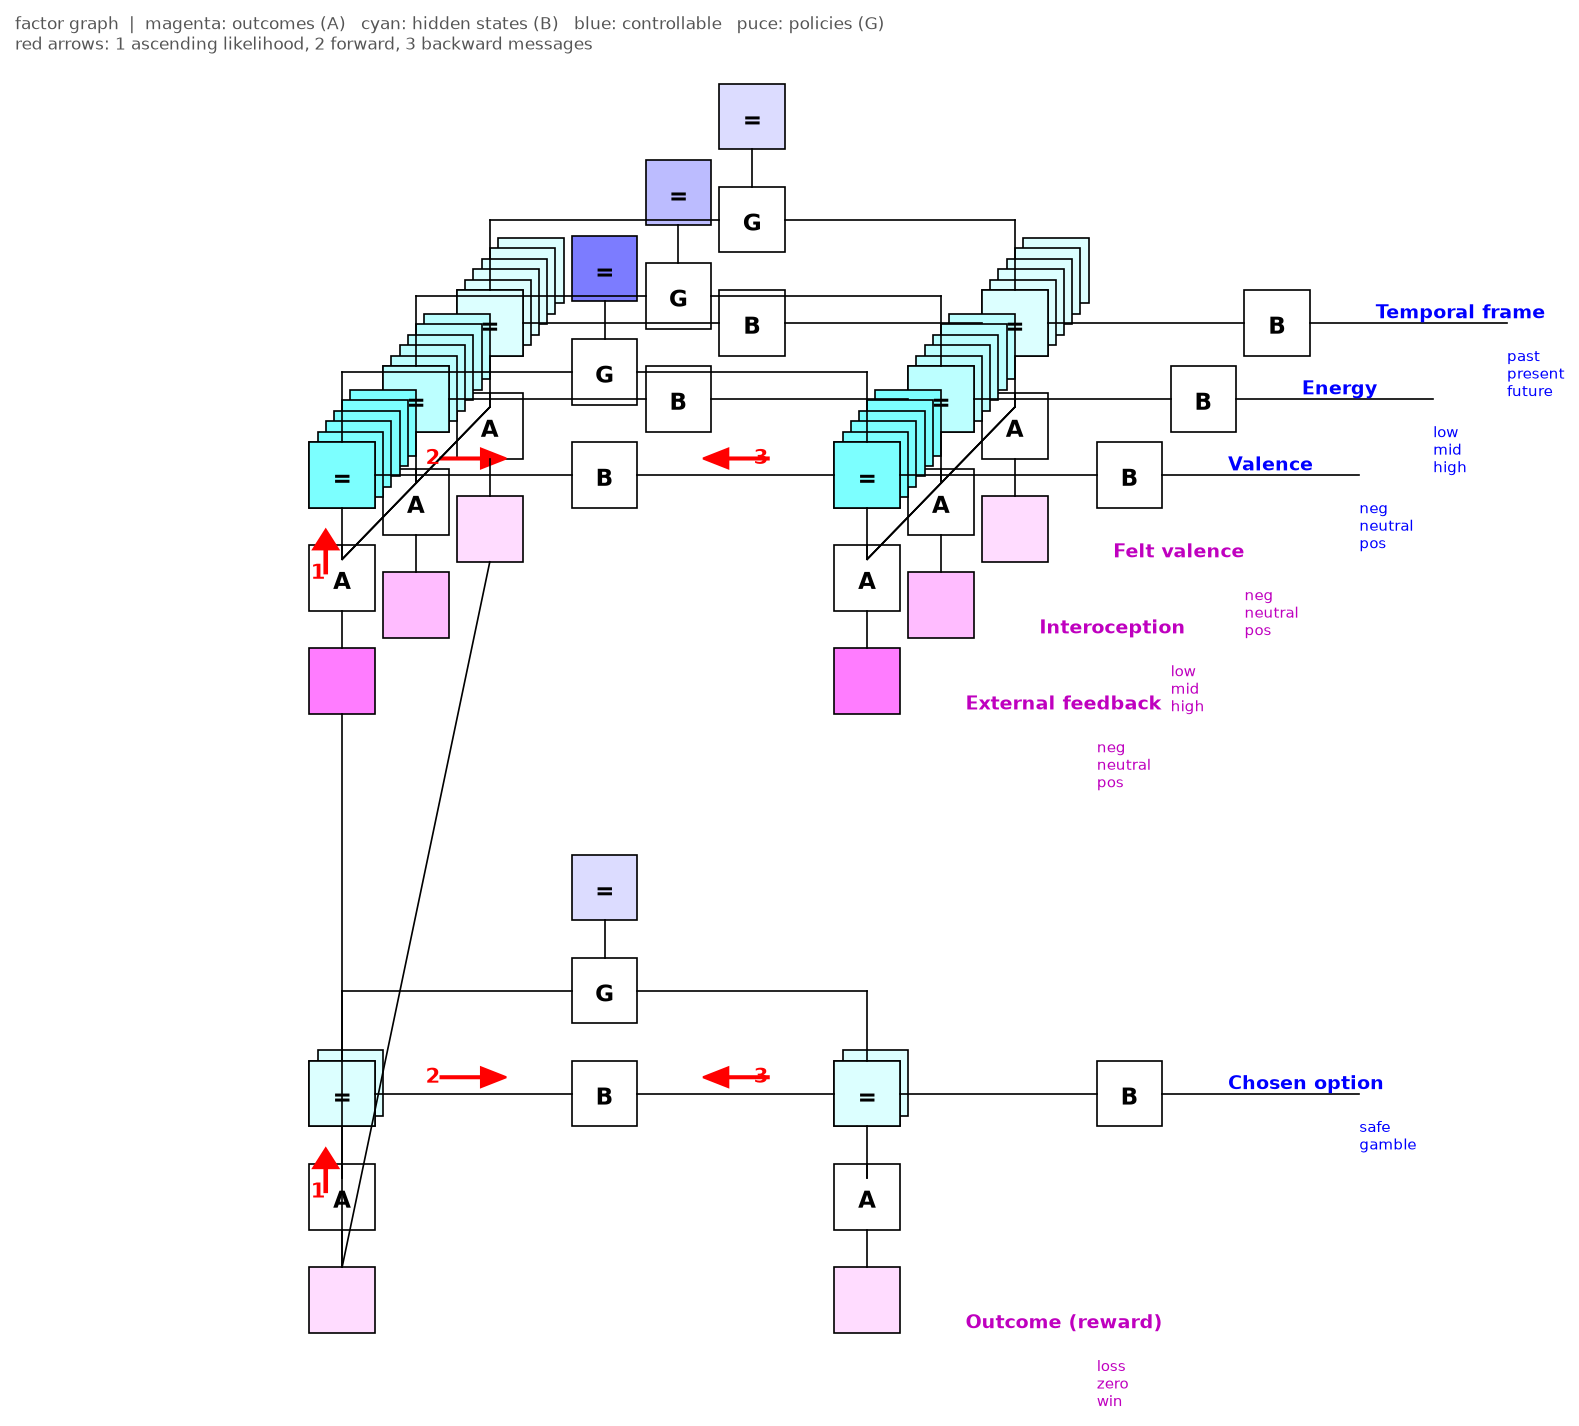
\includegraphics[width=0.9\textwidth]{figures/fig_gamble_affect_combined.png}
\caption{\textbf{The gamble task-model joined with the emotion model.} Two-level
factor graph of the subsumption test as actually run. The gamble task-model of
Figure~\ref{fig:gamble} (lower level: chosen option generating the reward outcome)
sits beneath the emotion model of Figure~\ref{fig:factorgraph} (upper level: valence,
energy, and temporal frame with their three modalities). The connecting edges carry
the task's reward outcome into the affect layer, directly as external feedback, and
via the three channels reading the task-model's inference dynamics as the felt-valence
observation. Each predecessor model in Table~\ref{tab:headtohead} corresponds to
retaining a single channel of this upper layer.}
\label{fig:gamblecombined}
\end{figure}

\begin{table}[htbp]
\centering\small
\caption{\textbf{Channel decomposition on the Rutledge gamble.} Each predecessor is
instantiated as its single affective channel over the same gamble task-model
(Figure~\ref{fig:gamble}); held-out $R^2$ for momentary happiness ($14{,}803$
participants, $96{,}624$ ratings), no expected value injected as a regressor. On a
single-shot gamble the backward (rate-of-change) and forward (policy-revision) channels
have no temporal dynamics to track, so their low scores are category-appropriate, not
defeats; the informative comparison is the present channel alone ($0.111$) against the
integrated readout ($0.144$), which reaches the reference ceiling.}
\label{tab:headtohead}
\begin{tabular}{llc}
\toprule
Model & Channel & Held-out $R^2$ \\
\midrule
Joffily \citep{joffily2013emotional} & backward (VFE rate) & 0.000 \\
Hesp \citep{hesp2021deeply} & forward (EFE charge) & 0.034 \\
Pattisapu \citep{pattisapu2024free} & present (RPE) & 0.111 \\
\textbf{Ours} & \textbf{all three} & \textbf{0.144} \\
\midrule
Happiness equation \citep{rutledge2014} & CR$+$EV$+$RPE (reference) & 0.146 \\
\bottomrule
\end{tabular}
\end{table}

\begin{figure}[htbp]
\centering
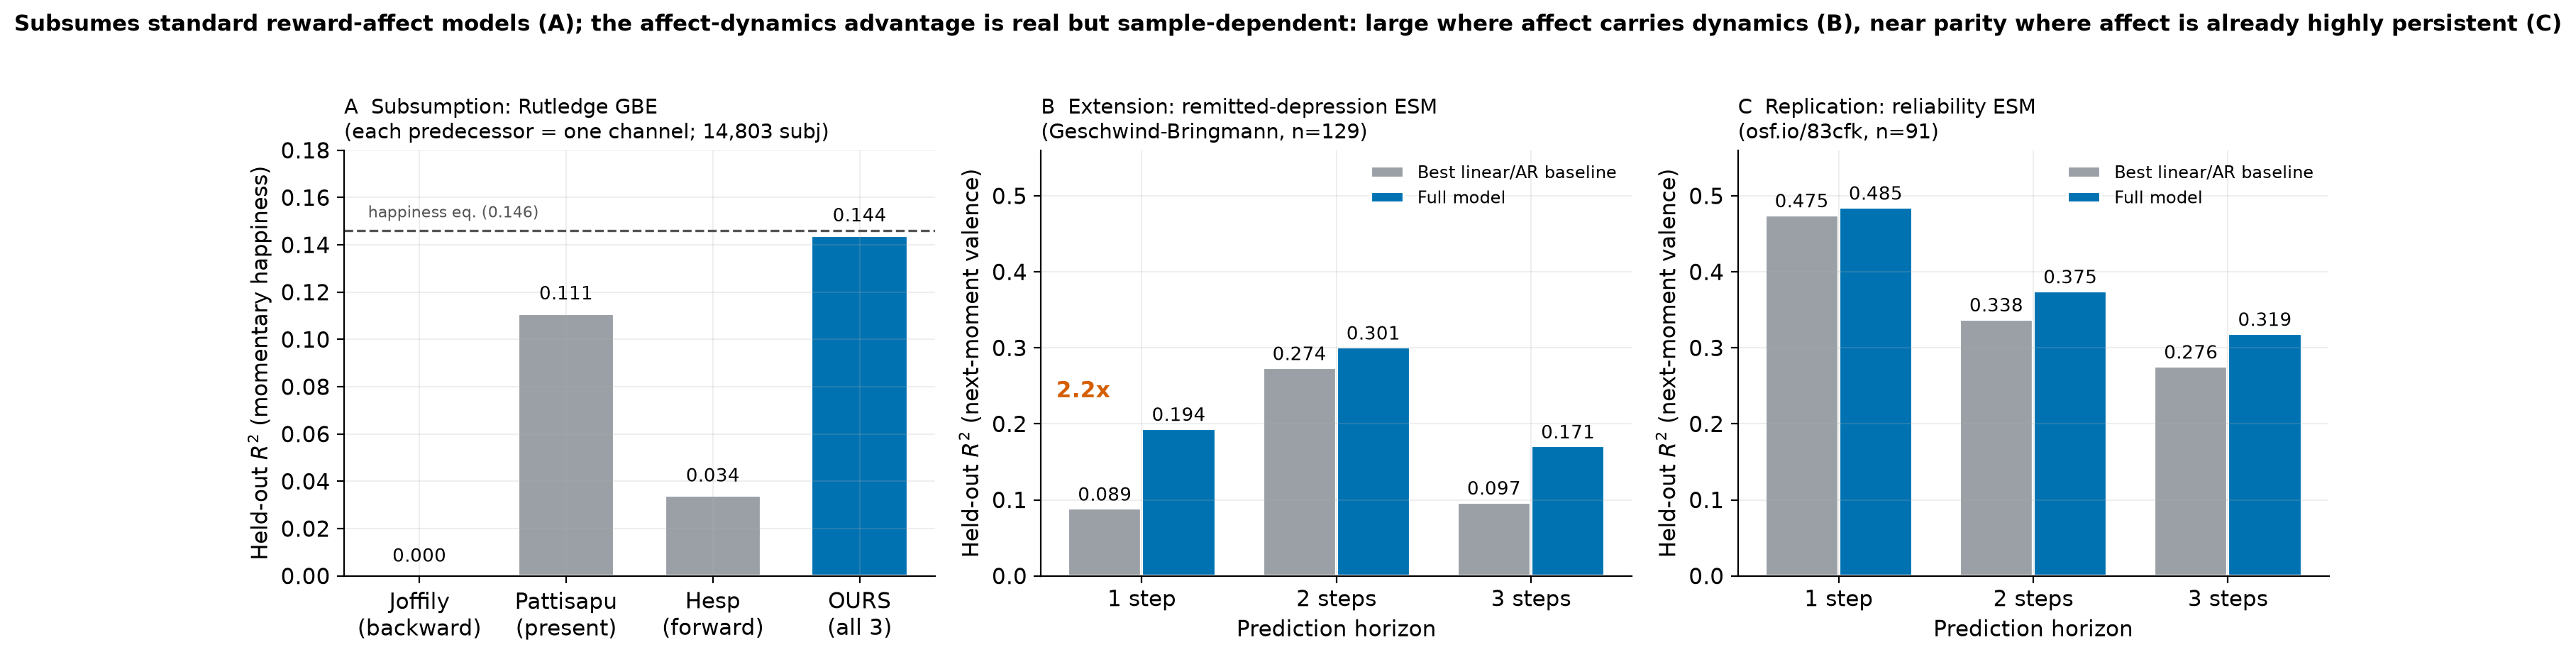
\includegraphics[width=\textwidth]{figures/fig_model_advantage.png}
\caption{\textbf{A general affect-readout framework.} (A) Channel decomposition (Rutledge GBE): each predecessor reconstructed as one channel over the same gamble
task-model; the present channel (Pattisapu 0.111) is the informative single-channel
comparison, the backward and forward channels being category-mismatched on a static
gamble, while integration reaches the reference ceiling (0.144 vs happiness equation
0.146, dashed). (B) On the remitted-depression ESM
sample, the full model reaches $2.2\times$ the held-out $R^2$ of the best
linear/autoregressive baseline at one step. (C) On an independent reliability ESM
sample the model leads at every horizon but by smaller margins, near parity at one
step, because affect there is already highly persistent (baseline $R^2=0.475$).
All held out across participants; Table~\ref{tab:esm}.}
\label{fig:advantage}
\end{figure}

\subsection{Extension: the full model predicts affect dynamics, on two samples}
Where the task has temporal structure, the temporal-frame factor earns its keep, and
we report the advantage on two independent experience-sampling samples rather than
one. In a remitted-depression ESM sample \citep{bringmann2013,geschwind2011} ($129$
participants held out; global parameters fitted on training participants and evaluated
on unseen ones), the full model predicts next-moment valence with held-out $R^2=0.19$
at one step versus $0.09$ for the best linear/autoregressive and event-regression
baselines, roughly double the explained variance at this horizon
(Figure~\ref{fig:advantage}B), with smaller leads at two and three steps. In a second,
independent reliability ESM sample (\texttt{osf.io/83cfk}, $91$ participants, no event
or worry items, so the model runs on valence alone), the model again leads at every
horizon, but the margins are modest and the one-step gap is near parity
(Figure~\ref{fig:advantage}C, Table~\ref{tab:esm}). The two samples differ in exactly
the way the framework predicts matters: in the reliability sample affect is already
highly persistent (baseline one-step $R^2=0.475$ versus $0.089$), leaving little
non-trivial dynamics for temporal machinery to capture, whereas the clinical sample's
more volatile affect is where the model helps most.

Component ablations locate the source of the advantage. Driving the model on valence
alone in the clinical sample changes almost nothing ($R^2=0.20$ at one step), so the
gain is not the event channel acting as a hidden regressor. Removing the
persistence-like valence-inertia term leaves the clinical-sample advantage intact
(the model still reaches $R^2=0.14$ at one step and $0.29$ at two steps with no inertia
at all, versus baselines $0.09$ and $0.27$); on the already-persistent reliability
sample the model sits at parity without inertia ($0.46$ vs $0.48$ at one step,
$0.34$ vs $0.34$ at two), consistent with there being little non-persistence structure
to capture there. Where the advantage exists, the model's own forward dynamics rather
than a persistence prior carry it. This holds
because the precision-gated prospection operator (\S\ref{sec:model}) keeps forward
rollouts calibrated to the agent's actual affective level rather than drifting toward a
fixed optimistic target. We do not claim a head-to-head reimplementation of each
predecessor here; the claim is that the integrated model outpredicts standard baselines
where affect carries non-trivial dynamics, and single components are insufficient.

\begin{table}[htbp]
\centering\small
\caption{\textbf{Affect-dynamics prediction on two independent ESM samples.} Held-out
$R^2$ for next-moment valence by prediction horizon, full model versus the best
linear/autoregressive baseline on identical inputs, 5-fold cross-validation with whole
participants held out. The reliability sample has no event items, so the model runs on
valence alone there.}
\label{tab:esm}
\begin{tabular}{llccc}
\toprule
Sample & Predictor & 1 step & 2 steps & 3 steps \\
\midrule
Remitted-depression ($n{=}129$) & baseline & 0.089 & 0.274 & 0.097 \\
\citep{bringmann2013,geschwind2011} & \textbf{full model} & \textbf{0.194} & \textbf{0.301} & \textbf{0.171} \\
\midrule
Reliability ($n{=}91$) & baseline & 0.475 & 0.338 & 0.276 \\
(\texttt{osf.io/83cfk}) & \textbf{full model} & \textbf{0.485} & \textbf{0.375} & \textbf{0.319} \\
\bottomrule
\end{tabular}
\end{table}

\subsection{Non-circular latent-state validation}
Driven only by valence and event inputs, the model's posterior \emph{future-frame}
belief covaries with an independently measured worry item it is never shown ($r=0.166$,
$n=11{,}712$). We read this as evidence that the frame belief couples to a
symptom-relevant affective signal, not that it recovers reported temporal orientation
as such; the direct orientation test below makes that distinction concrete.

\subsection{Direct temporal-orientation test}\label{sec:orientation}
The strongest test of the temporal-frame construct uses a dataset that labels the
orientation of thought itself. In an experience-sampling study with per-probe reports
of past- and future-directed thought alongside momentary valence
(\citealp{mulholland2023}; $n=101$, $1{,}458$ probes, CC BY-NC), the model's central
structural prediction holds and one of its default assumptions fails. The prediction
that past-framing carries negative valence under low positive-belief precision (the
RECALL/rumination branch) holds directly and within person: reported past-orientation
covaries negatively with momentary valence ($r=-0.23$ within person), and the effect
attenuates for people with higher trait positivity
($\beta_{\text{past}\times\text{trait}}=+0.06$), the direction the precision-gated
coupling predicts. The default that \emph{future}-framing is optimistic fails:
future-orientation is mildly negative in this unselected sample ($r=-0.07$). This
motivated the precision-gated FUTURATE operator of \S\ref{sec:model}, in which low
precision yields worry-type prospection. Two limits remain. First, the gating softens
the negativity of past-framing without reversing it, so the strong reading in which
rumination flips into positive narrative stabilisation overstates a real but weaker
effect. Second, driven on affect alone the model's latent frame does not \emph{recover}
reported orientation ($r\!\approx\!0$), because orientation is exogenous context the
model is never given; the validated claim is a frame-to-affect coupling, and testing
affect-to-frame recovery would require an orientation-carrying input channel.

\subsection{What does not improve prediction}
Across every dataset we tested, experience-sampling affect, two complete-feedback
counterfactual-learning tasks, a probabilistic reward task, and the large-scale
happiness data, and for both choice and affect targets, neither the hedonic
asymmetry ($c_{\text{pos}}\neq c_{\text{neg}}$) nor counterfactual depth improves
prediction. Both are redundant with reward-prediction signals. We
therefore present them as \emph{generative} and \emph{neurally/experientially}
grounded mechanisms rather than predictive components (Table~\ref{tab:claims}).

\begin{table}[htbp]
\centering\small
\caption{\textbf{What the framework can and cannot claim.} Predictive claims are
out-of-sample or out-of-model gains; generative claims are mechanisms that reproduce
phenomena and are neurally or experientially grounded but do not improve behavioural
prediction.}
\label{tab:claims}
\begin{tabular}{p{3.9cm}p{1.9cm}p{6.4cm}}
\toprule
Claim & Status & Evidence \\
\midrule
Multi-channel integration & predictive & recovers the happiness equation (Table~\ref{tab:headtohead}); outpredicts baselines on two ESM samples, $\sim$2$\times$ at one step where affect is volatile (Table~\ref{tab:esm}) \\
Latent temporal-frame state & predictive & future-frame belief tracks an unshown worry item ($r=0.17$) \\
Counterfactual emotion & generative & regret drives choice-switching ($t=10.4$); adds no choice or affect prediction \\
Hedonic asymmetry ($c_{\text{pos}}\!\neq\!c_{\text{neg}}$) & generative & blunted Reward Positivity, self-reported anhedonia; not recoverable from choice \\
\bottomrule
\end{tabular}
\end{table}

\section{Clinical mapping: a two-level account of depressive affect}\label{sec:clinical}
The framework draws a two-level picture of depressive affect and, more usefully,
predicts a dissociation between the levels that the data bear out. (i) A \emph{general}
reduction in reinforcement-learning rate/precision, present for both reward and
punishment learning. In our analysis of an open reward-and-punishment reversal-learning
dataset (\texttt{osf.io/2gq96}), depressed participants showed reduced learning rates in
\emph{both} conditions (Cohen's $d\approx-0.5$ to $-0.6$, not reward-selective), which
maps onto reduced overall precision and replicates the established mapping of anhedonia
onto reinforcement-learning parameters \citep{huys2013mapping}. (ii) A
\emph{reward-specific} valuation/reactivity deficit ($c_{\text{pos}}\!\downarrow$),
which converges with reward-specific ventromedial-frontal hypoactivation and blunted
Reward Positivity \citep{pirrung2025} and with self-reported anhedonia. The two levels
dissociate exactly as the model requires: $c_{\text{pos}}$ scales the \emph{value} an
outcome is assigned, while the learning rate governs how fast beliefs update, so a
sample can show reward-specific reactivity blunting (level ii) alongside a general
learning-rate deficit (level i) without contradiction, and the Pirrung sample does. The
value deficit is what Reward Positivity indexes; the learning deficit is what the
reversal task indexes. We label (ii) a model-derived prediction with convergent neural
and self-report support that awaits direct behavioural confirmation. A companion paper
develops the full bipolar phenotype characterisation.

\section{Discussion}\label{sec:discussion}
\subsection{What the integration buys}
The single move behind every result here is treating affect as a readout over a
task-specific model rather than as a model in its own right. That move has an empirical
consequence and a conceptual one. Empirically, the same three channels that recover the
happiness equation on a static gamble gain predictive power once the task carries
temporal structure, because only then does the temporal-frame factor have work to do.
Conceptually, prior single-channel accounts stop being rivals and become limiting
cases: each is what our readout reduces to when its task offers no dimension for the
other channels to read. Where a task lacks temporal structure the framework reduces to
the task-appropriate reward-affect model.

\subsection{Metastability as health}
Health is not a particular temporal configuration but the \emph{capacity to transition}
between configurations. The healthy agent visits multiple framing modes with a high
switching rate and short run lengths, metastability, in dynamical-systems terms.
Pathology is stickiness. Amplified reward sensitivity with impaired interoception locks
abstract forward framing on via absorptive narrative inertia; a habit prior locks RECALL
on while suppressing EFE-optimal escape. Restoring the ability to transition matters more than
correcting the balance between orientations.

\subsection{Attention as precision, and mood/emotion timescales}
Temporal framing extends attention-as-precision \citep{feldman2010attention} to the
temporal domain: $\mathbf B_{\text{frame}}$ matrices are temporal-attention operators,
and framing is deciding \emph{when} to attend. The framework sits at the interface of
the mood/emotion timescale hierarchy \citep{hesp2021deeply}. Individual frame
selections are within-trial (M4) phenomena; sustained biases are cross-trial (M5) mood.
This is where the thin (affect signals free-energy trajectories) and thick (affect is
the enactive force directing attention across horizons) readings of emotion meet.

\subsection{Limitations}
Emotion-level policy selection is single-step \citep{friston2018deep}; the frame is
categorical, not yet a continuous depth; the E-vector is fixed and not yet learned
\citep{watkins2008constructive}; and the model is single-agent, with dyadic temporal
co-regulation \citep{hinrichs2025temporal} left to future work. Empirically, the
per-channel head-to-head is on one dataset (Rutledge) and awaits replication; the
affect-dynamics advantage replicates across two ESM samples but with sample-dependent
margins. The direct temporal-orientation test (\S\ref{sec:orientation}) validates the
frame-to-affect coupling but also shows its two current limits: the model does not
invert reported orientation from affect alone (it is not given orientation-carrying
input), and precision gating attenuates rather than reverses the negativity of
past-framing. Grounding the frame in an orientation-carrying observation channel, so
the latent frame can be tested for recovery and not only coupling, is the most valuable
next step.

\bibliographystyle{plainnat}
\bibliography{references}
\end{document}
